\section{Event selection}
\label{sec:objects}

In this section, the selections applied to the physics objects used in the analysis are presented and motivated by performance and validation plots. Background events are represented as coloured histograms: \Z + jets events in light blue, \W + jets events in violet, \ttbar events in yellow, single-top events in orange, diboson (or \VV) events in blue, multi-jet (QCD) events in gray. Background uncertainties are displayed as black shaded areas. Signal samples are represented as coloured shaded histograms: the kind of signal (graviton or \Wp), the mass and cross-section of the considered resonance are reported in the legend. Data are represented with black markers, with their corresponding Poissonian uncertainty bars. If data are displayed, the data-MC ratio is reported per each bin in the bottom panel, along with the overall data-MC ratio calculated in the whole spectrum and the scores of $\chi^2$ and Kolmogorov-Smirnov goodness-of-fit tests.
%%The objects are selected according to the standard Run2 reccomendations provided by the various POGs for the Summer16 (25ns) MiniAOD-v2 (Moriond reccomendations).
%The version of CMSSW used for the analysis is {\tt CMSSW\_8\_0\_25}.

\subsection{Vertex and Pile-up}
Due to the pile-up effect, several vertices are typically reconstructed in one event. The primary vertex of the event is defined as the one with the highest sum of transverse momenta $\sum \pt^2$ of clustered physics objects associated to it, which passes the following selections:
\begin{itemize}
  \item number of degrees of freedom $N_{DoF}>4$
  \item vertex position along the beampipe $|z_{vtx}|<24\cm$
  \item vertex distance with respect the beam pipe $d_0<2\cm$
\end{itemize}
where $z_{vtx}$ and $d_0$ are the distance along and perpendicular to the beam line of the vertex with respect the nominal interaction point $(0,0,0)$.

\noindent The Monte Carlo samples listed in sec.~\ref{sec:samples} are generated simulating the pile-up conditions, as expected in the 25 ns bunch crossing pile-up scenario. Nevertheless, the MC pile-up description does not match exactly the conditions in data, and there is therefore the need to reweight the simulated events in order to improve the agreement with the data. 

\noindent The MC samples are reweighted assuming a total inelastic cross section of $\sigma_{in} = 69\,200 \mu b$. The comparison between the distributions of primary vertices in data and MC after the pile-up reweighting is applied is shown in fig.~\ref{fig:npv} for an event selection (called inclusive selection, described in sec.~\ref{sec:datamc_comp}) requiring large amount of \met recoiling against an AK8 fat jet~(tab.~\ref{tab:sel}).
 
 \begin{figure}[!htb]
  \centering
    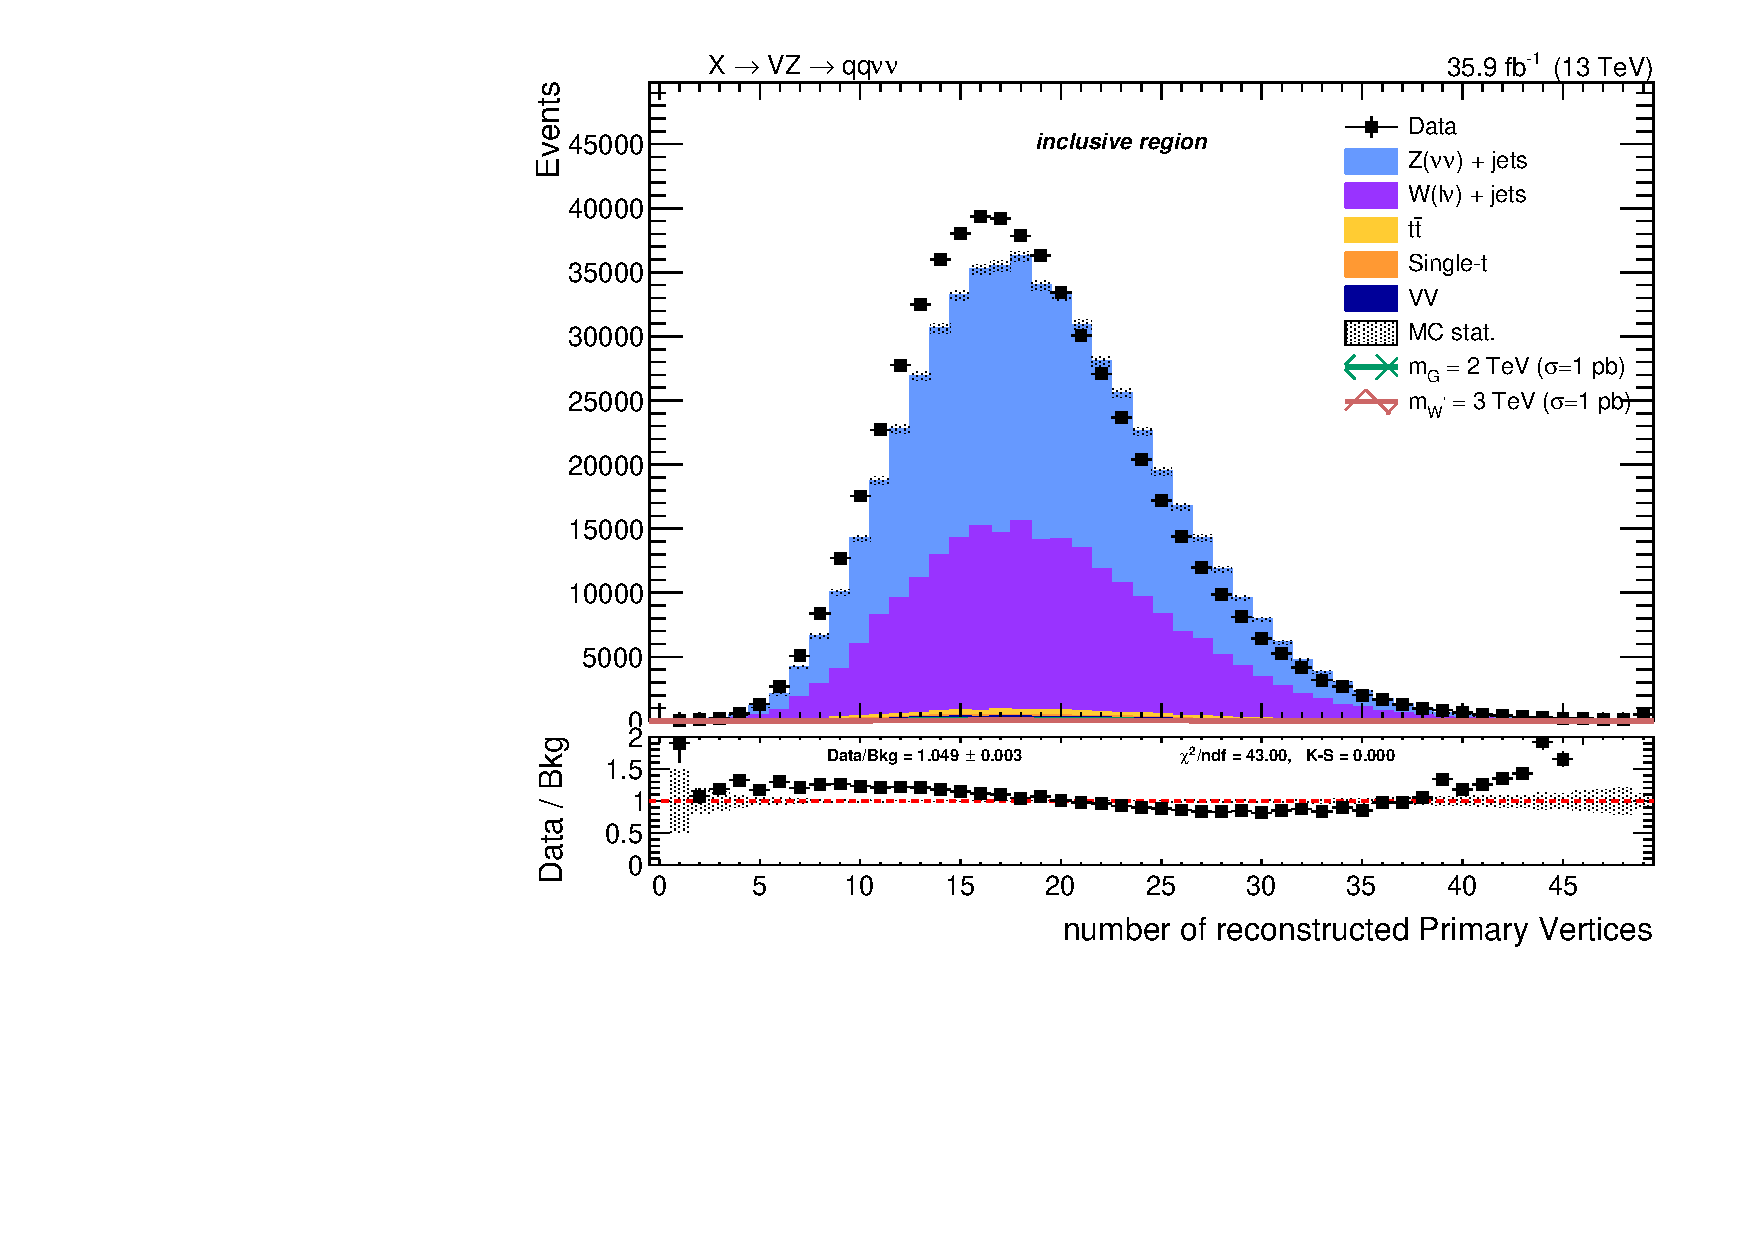
\includegraphics[width=.495\textwidth]{plots/v9_thesis/XVZnnInc/nPV.pdf}
  \caption{Primary vertices distributions in data and MC samples, after reweighting.}
  \label{fig:npv}
 \end{figure}


\subsection{Electrons}\label{ssec:electrons}
%{\color{red} How the electrons are reconstructed: The electron identification variables that have been found to be the most powerful, and are used in the selection, are: the energy-momentum match between the seed cluster and the trackE seed/pin, the variables measuring spatial matching between the track and the supercluster, ∆ηin and ∆φin, the supercluster η width,σiη iη(as taken from the covariance matrix using logarithmic weights), and the hadronic leakage variable H/E. The supercluster η width is to a very good approximation unaffected by the spreading due to the magnetic field of the showering in the tracker material.\\ Isolation variables are computed in three sub-detectors: the tracker, the ECAL, and the HCAL. Transverse energy/momentum sums are evaluated in regions of ∆R<0.3. As electrons undergo bremsstrahlung energy loss in the tracker material, care is taken to remove from the isolation sums the contributions from bremsstrahlung photons and possible resulting conversion electrons.}

Electrons considered in this analysis, reconstructed from energy deposits in the ECAL matched to tracks reconstructed in the silicon tracker, are required to pass the particle flow criteria, and to fall in the ECAL pseudorapidity fiducial range ($|\eta|<2.5$). The electron identification is defined with a ``cut-based'' approach. In the isolation definition, the effect of pile-up is considered by taking into account the energy deposits in the calorimeter, estimated through the so-called \emph{$\rho$-area} method, by subtracting the median energy density in the event $\rho$ multiplied by the electron energy deposits effective area. The isolation value is computed in a $\Delta$R cone of 0.3 centered along the lepton direction.

\noindent Since in this analysis aims at a final state without any lepton, every electron identified with the looser cut-based criteria (\emph{veto Id}) and transverse momentum $\pt > 10$ GeV is vetoed. The detailed set of cuts to define a \emph{veto Id} cut-based electron are reported in tab.~\ref{tab:EGcutBar}; this set of selections allow to identify an electron with an efficiency of $\sim 95$\%. The supercluster width is indicated as $\sigma_{i\eta i\eta}$; $\Delta \eta_{in}^{seed}$ and $\Delta \varphi_{in}$ are the difference in $\eta$ and $\varphi$ between the track position as it is measured in the inner layer, and then extrapolated to the interaction vertex and to the calorimeter, and the $\eta$ of the seed cluster or the $\varphi$ of the supercluster; $H/E$ is the hadronic leakage, \textit{i.e.} the ratio of the hadronic energy of the calorimetric towers to the electromagnetic energy of the electron supercluster; \emph{relIso} indicates the relative isolation calculated with the effective area approach; $1/E - 1/p$ is the difference of the inverse of the energy and the momentum; $d_0$ and $d_z$ are the transverse and longitudinal impact parameters. A dedicated conversion veto is applied to mitigate the effects of electrons undergoing bremsstrahlung in the silicon detector.

\begin{table}[htb]
 \centering
\caption{Electron cut-based selection for 25 ns bunch spacing conditions. EB: barrel cuts (~$|\eta_\text{supercluster}| \leq 1.479$~); EE: endcap cuts ( $|\eta_\text{supercluster}| > 1.479$)}
    \begin{tabular}{l|ccc}
    Electrons                   &        & \multicolumn{2}{c}{\emph{Veto Id}}\\
                                &        & EB      & EE     \\
 \hline
 \hline
    $\sigma_{i\eta i\eta} $     & $ < $  &0.0115   &0.037  \\
    $\Delta \eta_{in}^{seed}$   & $ < $  &0.00749  &0.00895 \\
    $\Delta \varphi_{in} $      & $ < $  &0.228    &0.213   \\
    $H/E $                      & $ < $  &0.356    &0.211   \\
    relIso (Effective Area)                 & $<$    &0.175    &0.159   \\
    $|1/E - 1/p|$               & $ < $  &0.299    &0.15    \\
    $|d_0|$                     & $ < $  &0.05     &0.10   \\
    $|d_z|$                     & $ < $  &0.10     &0.20   \\
    missing hits                & $\leq$ &2        &3       \\
    conversion veto             &        &  yes    &yes     \\
    
\end{tabular}

\label{tab:EGcutBar}
\end{table}

%Per-event data-MC scale factors for electron identification are calculated and applied in the analysis.
%\clearpage

\subsection{Photons}
As in the case of electrons, a photon veto is applied in the analysis both for the signal and the control regions. Events are rejected if they contains one (or more) photon with $\pt > 15$ GeV , $|\eta| < 2.5$, passing the \emph{loose} cut-based photon Id, whose definition is reported in tab.~\ref{tab:PhotonId}. The isolation cuts (using the $\rho$-area method for the mitigation of the pile-up) and conversion-safe veto are applied. The isolation value is computed in a $\Delta R$ cone of 0.3 and it is corrected for pile-up by subtracting the event-by-event energy density ($\rho$) times the photon energy deposits effective area.

 \begin{table}[htb]
  \centering
  \caption{Photon cut-based selection for 25 ns bunch spacing conditions. EB: barrel cuts ( $|\eta_\text{supercluster}| \leq 1.479$); EE: endcap cuts ( $|\eta_\text{supercluster}| > 1.479$)}\label{tab:PhotonId}
     \begin{tabular}{l|ccc}
     Photons                                   &       & \multicolumn{2}{c}{\emph{Loose Id}}\\
                                               &       & EB      & EE  \\
  \hline
  \hline
     $H/E $                                    & $ < $ &0.0597   & 0.0481      \\
     $\sigma_{i\eta i\eta} $                   & $ < $ &0.01031  & 0.03013   \\
     PF ch.had.iso.($\rho$-corr)               & $ < $ &1.295    & 1.011   \\
     PF neu.had.iso.($\rho$-corr)              & $ < $ &$10.910+0.0148\pt+0.000017\pt^2$    &$5.931+0.0163\pt+0.000014\pt^2 $   \\
     PF photon iso.($\rho$-corr)               & $ < $ &$3.630+0.0047\pt$                 &$6.641+0.0034\pt $   \\
     conversion veto                           &       & yes     &yes     \\
 \end{tabular}

 \end{table}

%Scale factors for photon identification (including isolation) are provided by Egamma POG, derived for 80X (Moriond 17 recommendation), that can be found in~\cite{EGammaPOG_ele_SF}.

\subsection{Muons}\label{ssec:muons}

%Tracker Muon reconstruction is more efficient than the Global Muon reconstruction at low momenta, $\pt \lesssim 5 \GeV$, because it requires only a single muon segment in the muon system, whereas Global Muon reconstruction is designed to have high efficiency for muons penetrating through more than one muon station and typically requires segments in at least two muon stations. Thanks to the high tracker-track efficiency and a very high efficiency of reconstructing segments in the muon system, about 99\% of muons produced in $pp$ collisions and having sufficiently high momentum are reconstructed either as a Global Muon or a Tracker Muon, and very often as both. Muons reconstructed only as standalone-muon tracks have worse momentum resolution and less favorable collision muon to cosmic-ray muon ratio than the Global and Tracker Muons and are usually not used in physics analyses.

The minimal criteria to define a muon is that it must be identified by the particle flow algorithm, and should be reconstructed either as a global muon or as a tracker muon (sec.~\ref{ssec:physicsobjects}). The muon isolation is defined in a cone with a radius of $\Delta R=0.4$ centered along the lepton direction. In the analysis event selection, all muons identified with the loosest criteria previously described, \pt over 10 GeV, PF isolation below 0.25, $\eta<|2.4|$ are vetoed.
 
%Scale factors for muon identification and isolation are centrally provided as a function of the muon \pt and $\eta$ by the Muon POG~\cite{MuonSF}, and are applied consistently in the analysis.


\subsection{Taus}\label{ssec:tau}
The presence of hadronically decaying taus acts as a veto for the events both in the signal and in the control regions, in order to suppress electroweak backgrounds. The selection criteria for taus are $\pt > 18$ GeV and $|\eta| < 2.3$. Loose identification criteria of the hadronic tau reconstruction algorithms are required and applied in order to identify possible tau candidates.


\subsection{Jets}\label{ssec:jets}
In this analysis, jets are considered if the corrected \pt is larger than 30 \GeV for AK4 jets, and larger than 200 \GeV for AK8 jets, and lie in the tracker acceptance ($|\eta|<2.4$). The requirement on AK8 jets transverse momentum is motivated by the fact that $\pt = 200$ \GeV is the minimum kinematical threshold ensuring to enclose the lighter hadronically decaying vector boson (namely, the \W boson) in the jet cone. Additionally, AK4 jets are required to pass \emph{loose} jet identification requirements, AK8 are required to pass \emph{tight} jet identification requirements defined in tab.~\ref{tab:JetId}. AK8 jets are used to reconstruct the hadronically decaying electroweak boson candidate, whilst AK4 jets are used to suppress the contribution of top and QCD background events. Jet energy corrections are applied to AK4 and AK8 CHS jets. Fig.~\ref{fig:n_AK8}-~\ref{fig:AK8jet_eta} show the data/simulation comparison after the analysis selections~(tab.~\ref{tab:sel} without Top cleaning and Event cleaning).

\begin{table}[htb]
 \centering
 \caption{ \emph{Loose} and \emph{Tight} jet identification requirements for 25 ns bunch spacing conditions.\label{tab:JetId}}
 \begin{tabular}{l|cc}
Particle flow jet ID                       & \emph{Loose}   & \emph{Tight}   \\
\hline
 \hline
Neutral Hadron Fraction         & $< 0.99  $     & $< 0.90  $    \\
Neutral EM Fraction             & $< 0.99  $     & $< 0.90  $\\
Number of Constituents          & $> 1     $     & $> 1     $\\
Muon Fraction                   & \--            & \-- \\
\hline
\multicolumn{3}{l}{Additionally, for $|\eta| < 2.4$ } \\
\hline
Charged Hadron Fraction         & $> 0   $& $> 0   $\\
Charged Multiplicity            & $> 0   $& $> 0   $\\
Charged EM Fraction             & $< 0.99$& $< 0.99$\\
 \end{tabular}

\end{table}

\begin{figure}[!htb]
  \begin{center}
    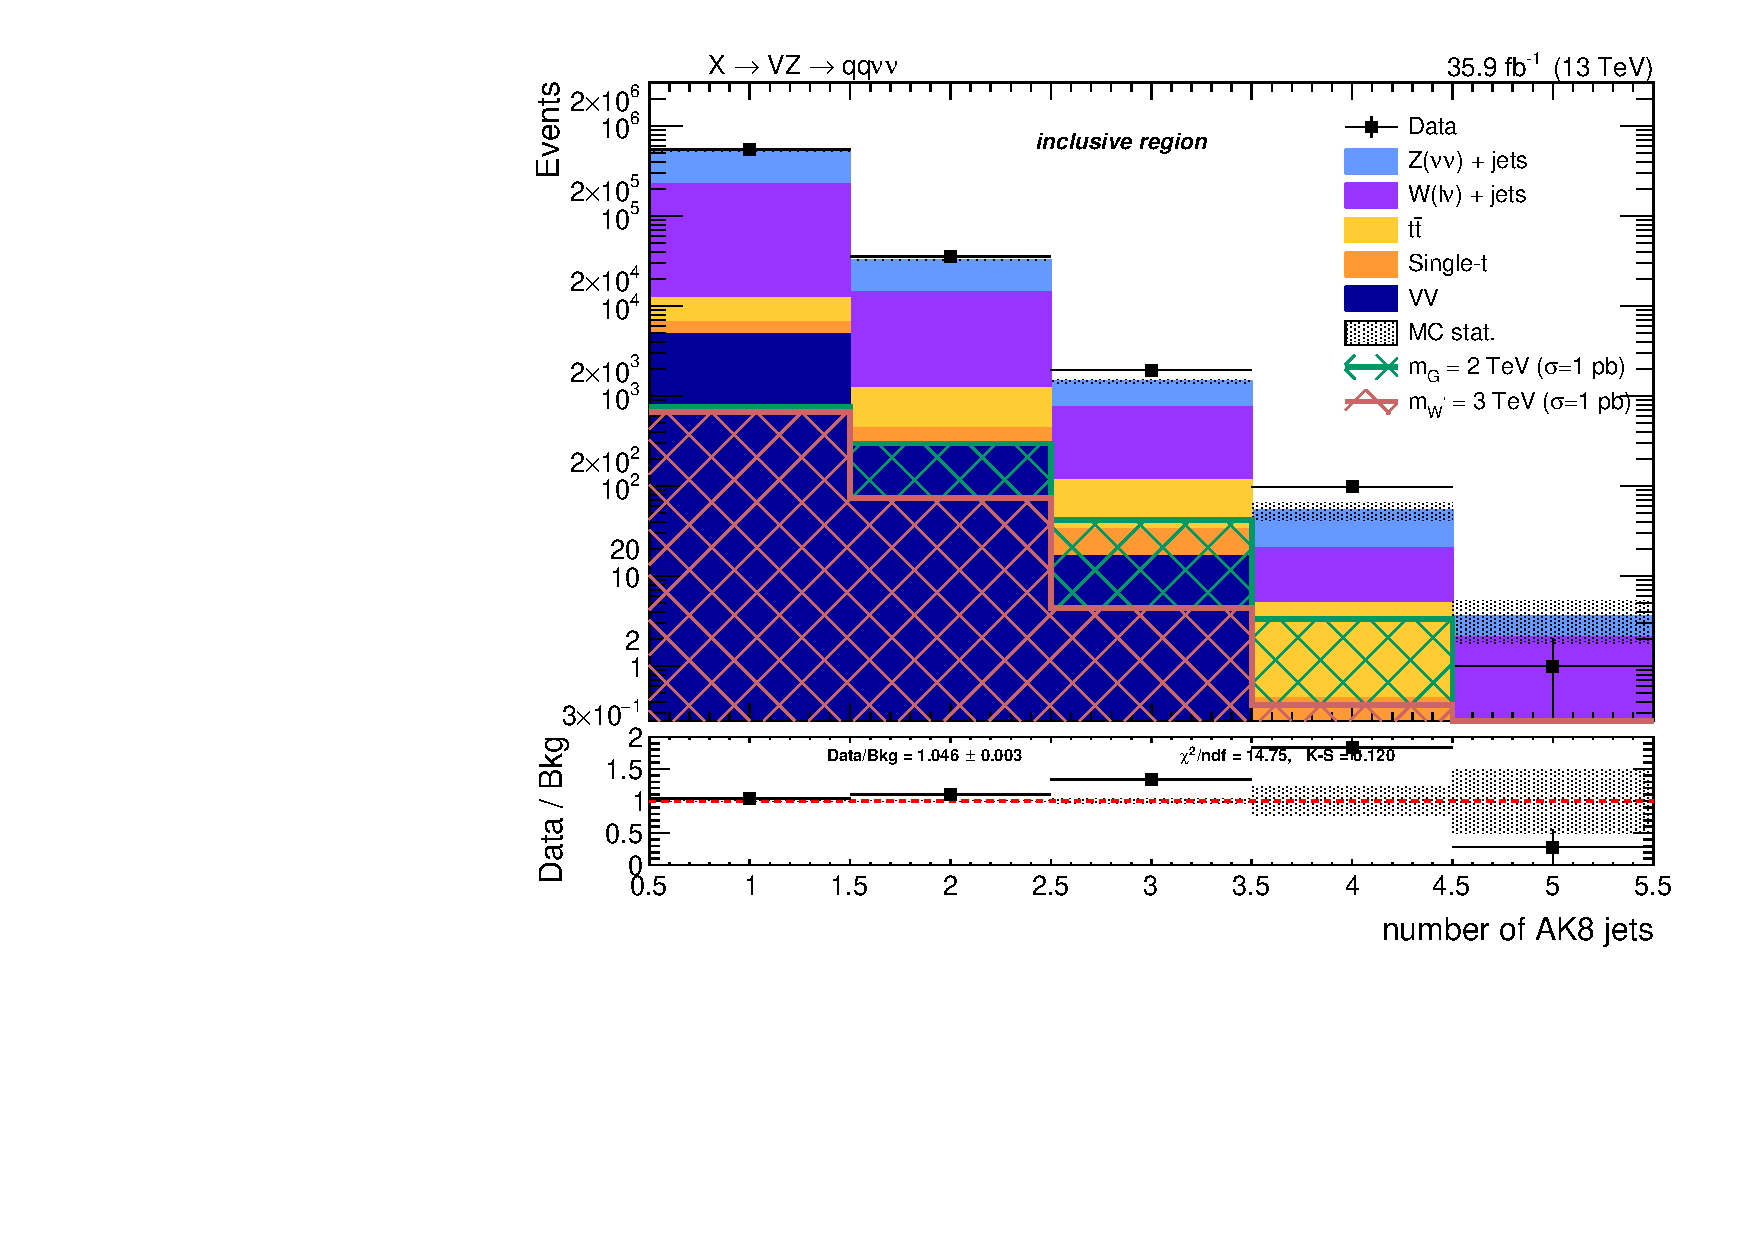
\includegraphics[width=.495\textwidth]{plots/v9_thesis/XVZnnInc/nFatJets.pdf}
  \end{center}
  \caption{Number of reconstructed AK8 jets after inclusive selections.}
  \label{fig:n_AK8}
\end{figure}

\begin{figure}[!htb]
  \begin{center}
    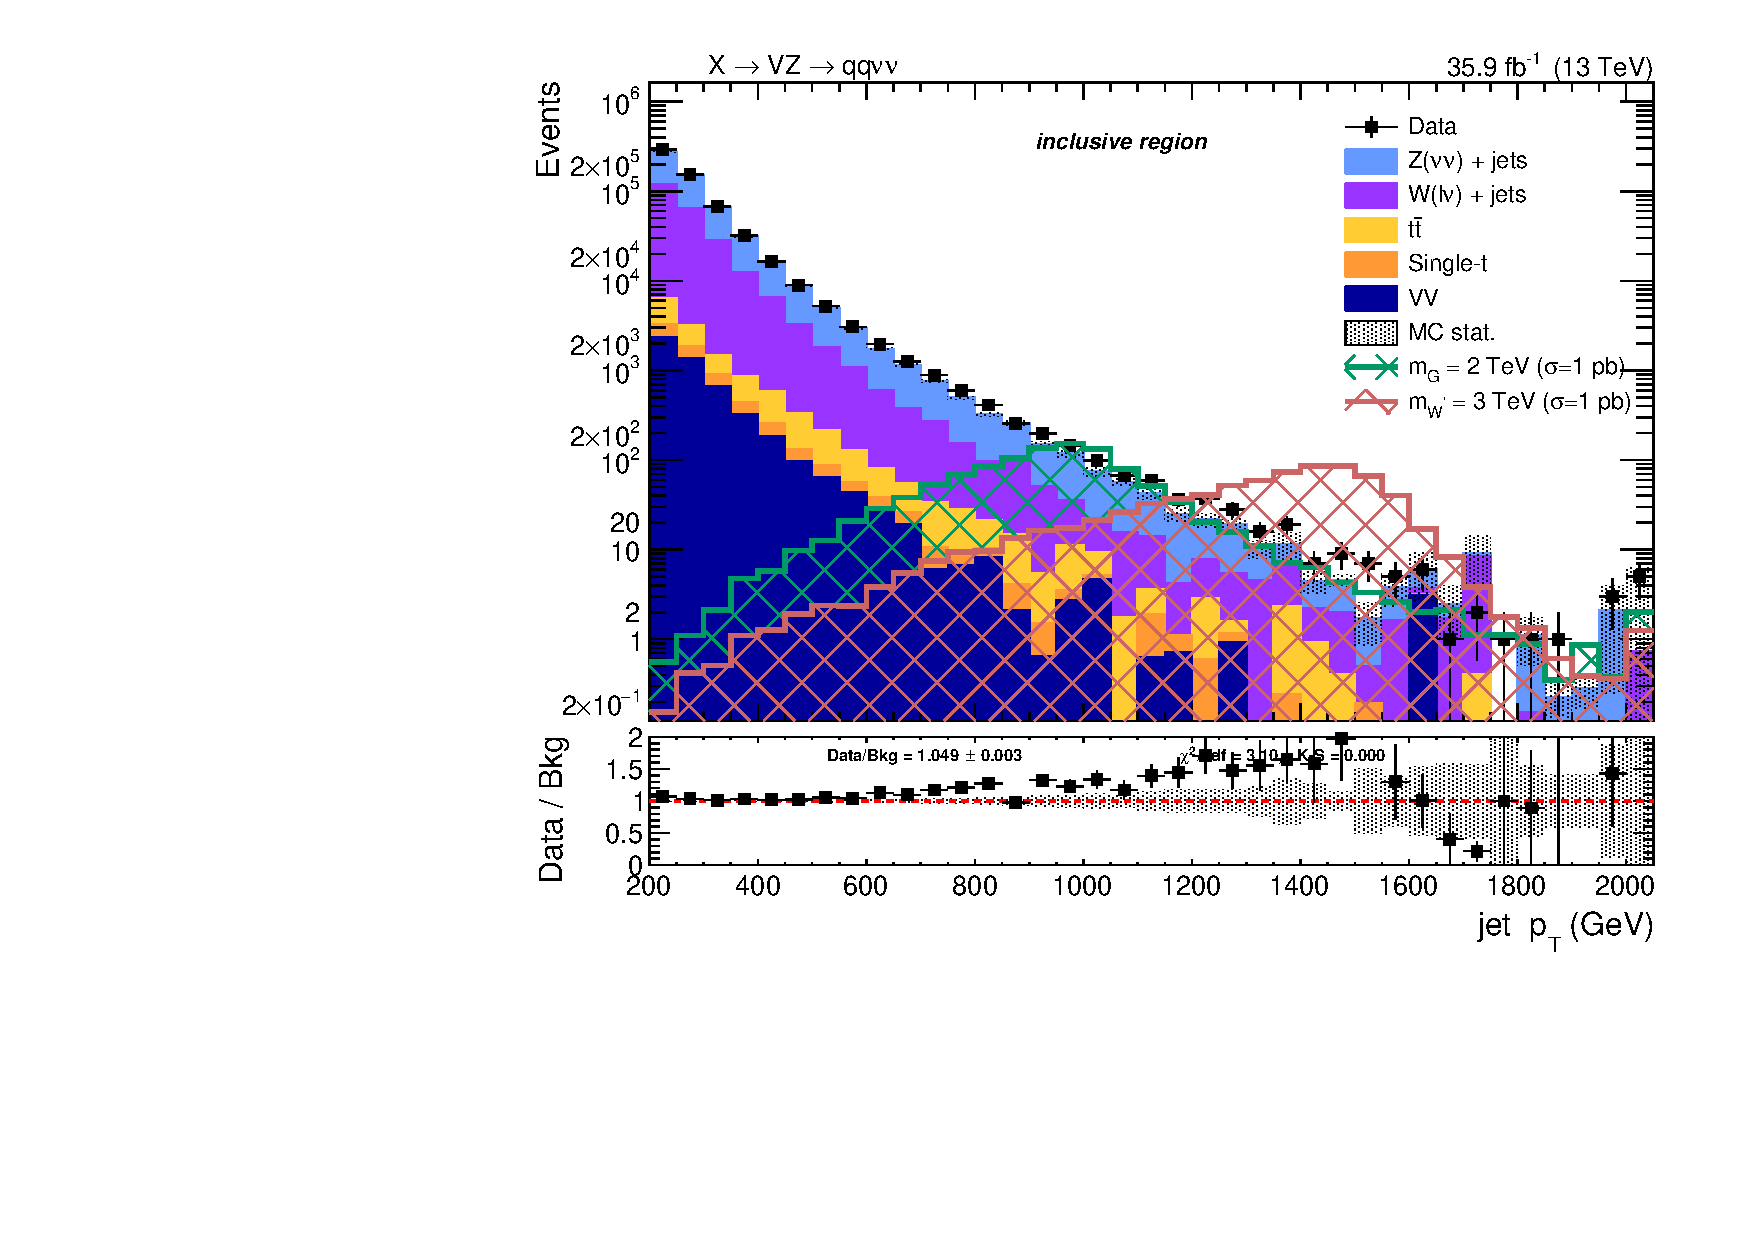
\includegraphics[width=.495\textwidth]{plots/v9_thesis/XVZnnInc/FatJet1_pt.pdf}
  \end{center}
  \caption{Leading AK8 jet \pt spectrum after inclusive selections.}
  \label{fig:AK8jet_pt}
\end{figure}

\begin{figure}[!htb]
  \begin{center}
    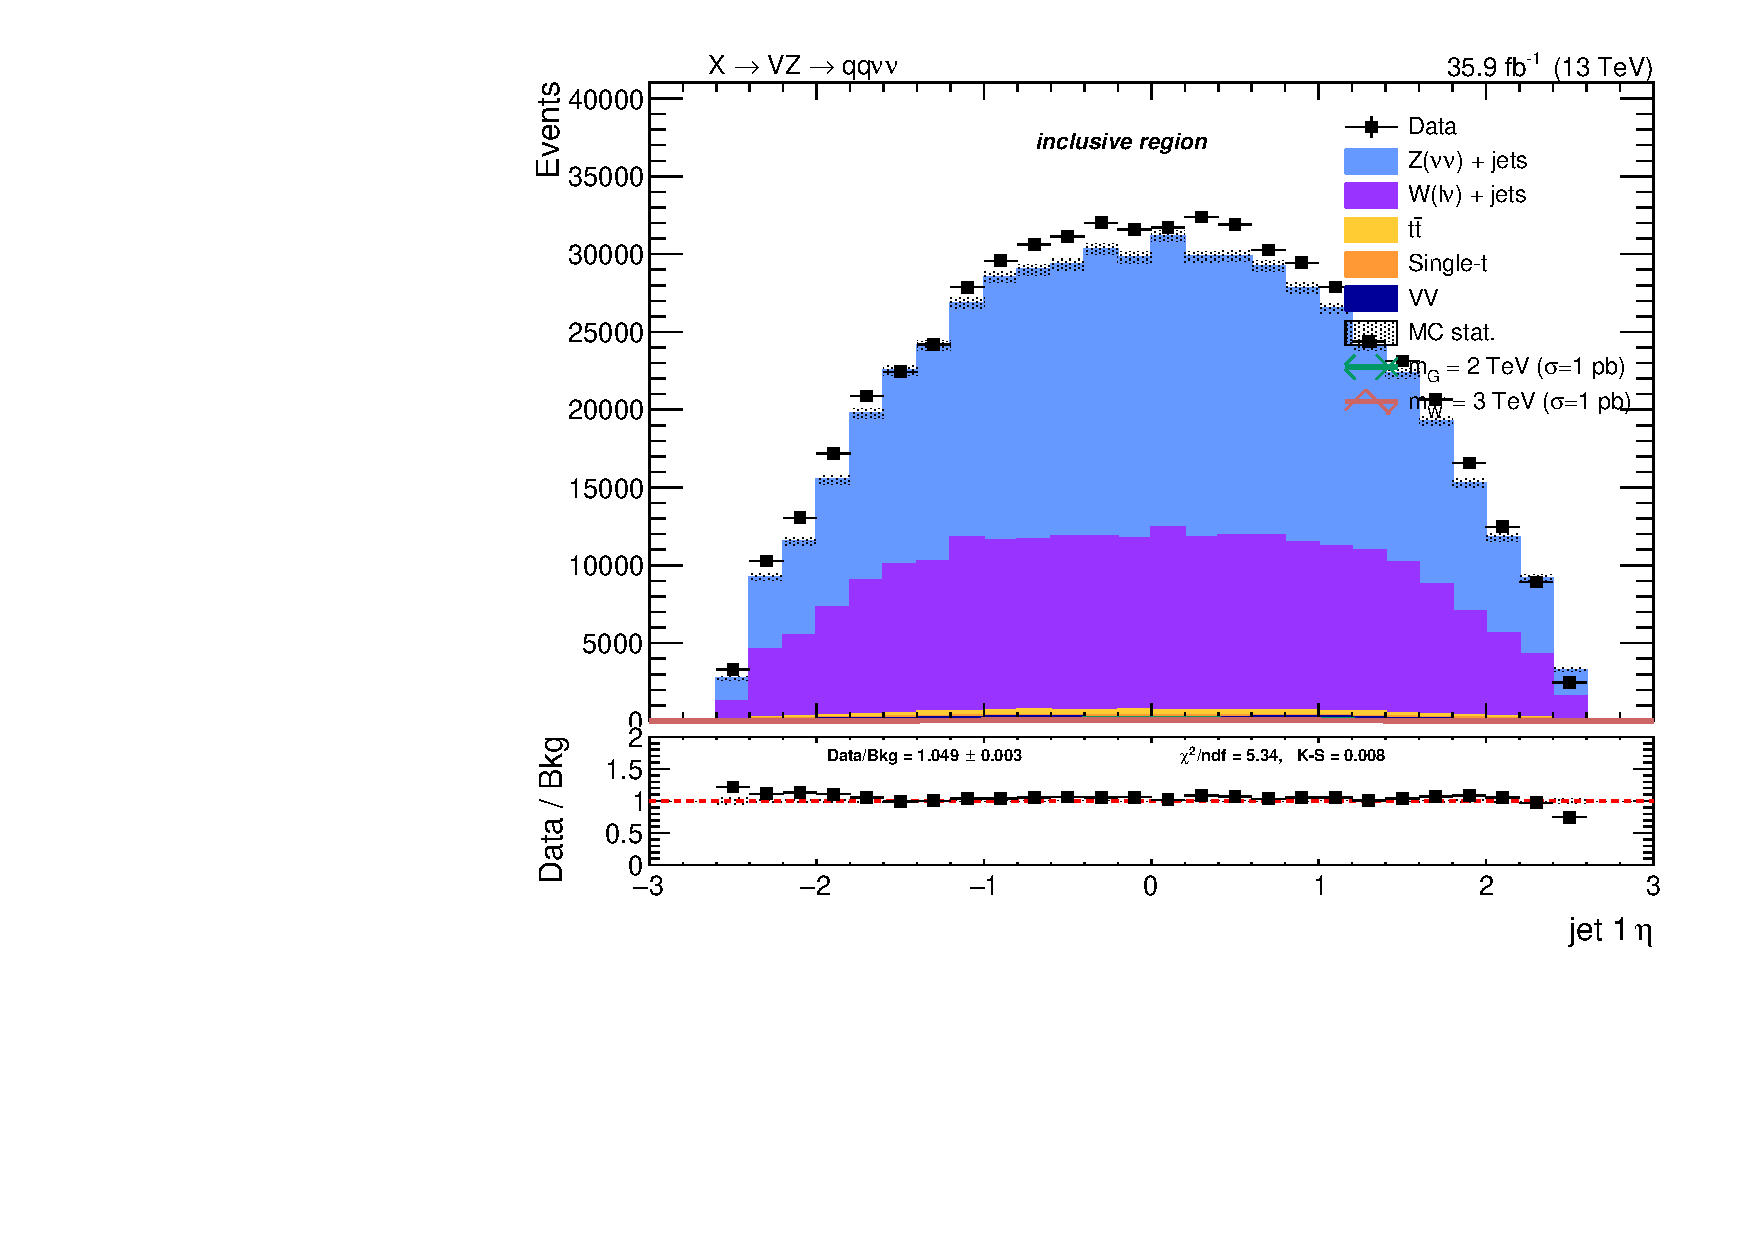
\includegraphics[width=.495\textwidth]{plots/v9_thesis/XVZnnInc/FatJet1_eta.pdf}
  \end{center}
  \caption{Leading AK8 jet $\eta$ spectra after inclusive selections.}
  \label{fig:AK8jet_eta}
\end{figure}

\noindent Since it has been measured that the jet energy resolution (JER) is not the same in data and MC, an additional smearing is applied in simulation, in order to get a better agreement. There are two independent ways to get the smearing. The scaling method rescales the corrected four-momentum of a reconstructed jet by a factor
\begin{equation}
c_{\text{JER}} = 1 + (s_{\text{JER}} - 1) \frac{p_T - p_T^{\text{gen}}}{p_T},
\end{equation}
where \pt is the transverse momentum of the jet, $p_T^{\text{gen}}$ is the transverse momentum of the generator level particle corresponding to the reconstructed jet, and $s_{\text{JER}}$ is the data-simulation resolution scale factor. The factor $c_{\text{JER}}$ is positively defined, hence, when negative, it is set equal to zero. %This method only works if a well-matched particle-level jet is present and can result in a large shift of the response otherwise.
The generator level particle and a reconstructed jet are defined as matched if:
\begin{equation}
\begin{split}
& \Delta R < R_{0} / 2, \\
&  |p_T - p_T^{\text{gen}}| < 3 \times \sigma_{\text{JER}} \times p_{T}, \\
\end{split}
\end{equation}
where $R_{0}$ is the jet clustering parameter and $\sigma_{\text{JER}}$ is the relative \pt resolution measured in simulation.

\noindent The alternative approach is the stochastic smearing, and it does not require the matching with the generator level particle. The jet four-momentum is rescaled by a factor
\begin{equation}
c_{\text{JER}} = 1 + \mathcal{N}(0, \sigma_{\text{JER}}) \sqrt{\text{max}(s_{\text{JER}}^2 - 1, 0)},
\end{equation}
where $\sigma_{\text{JER}}$ is the relative \pt resolution in simulation, $s_{\text{JER}}$ is the data-simulation scale factor, and $\mathcal{N}(0, \sigma)$ 
is a random number extracted from a gaussian normal distribution, whose mean is zero and variance $\sigma^2$. Scaling factor $c_{\text{JER}}$ is positively defined.% This method only allows to degrade the resolution.

\noindent The smearing procedure adopted in this analysis is the hybrid method: when a matching jet at generator level is found, the scaling method is adopted, else the stochastic smearing is chosen. The smearing coefficients (scale factors, SF) as a function of the jet $\eta$ and their uncertainties are reported in tab.~\ref{tab:smear} for 2016 data~\cite{CMS-DP-2016-020}.

\begin{table}[!htb]
  \centering
  \caption{Data-simulation jet smearing coefficients and their corresponding uncertainties.}
  \begin{tabular}{l|c}
    Jet $\eta$ & Smearing SF \\
    \hline
    \hline
    $0.0-0.5$ & $1.109 \pm 0.008$ \\
    $0.5-0.8$ & $1.138 \pm 0.013$ \\
    $0.8-1.1$ & $1.114 \pm 0.013$ \\
    $1.1-1.3$ & $1.123 \pm 0.024$ \\
    $1.3-1.7$ & $1.084 \pm 0.011$ \\
    $1.7-1.9$ & $1.084 \pm 0.011$ \\
    $1.9-2.1$ & $1.140 \pm 0.047$ \\
    $2.1-2.3$ & $1.067 \pm 0.053$ \\
    $2.3-2.5$ & $1.177 \pm 0.041$ \\
    $2.5-2.8$ & $1.364 \pm 0.039$ \\
    $2.8-3.0$ & $1.857 \pm 0.071$ \\
    $3.0-3.2$ & $1.328 \pm 0.022$ \\
    $3.2-5.0$ & $1.16  \pm 0.029$ \\
  \end{tabular}
  

  \label{tab:smear}
\end{table}

\subsection{Jet mass}\label{ssec:jetmass}

The jet mass is the main observable in distinguishing a \V jet from a jet produced by colour interaction (QCD jets). Jet grooming procedure consists in the suppression of uncorrelated underlying event, pile-up and soft radiation from the jet: it improves the signal and background discrimination, by pushing the jet mass for QCD jets towards lower values of the spectrum, while maintaining the jet mass for \V-jets around the electroweak boson mass window.

\noindent The grooming technique of the analysis relies on the ``soft drop declustering'' algorithm, a jet substructure technique that recursively removes soft wide-angle radiation from a jet~\cite{Larkoski:2014wba}, in order to mitigate the contaminations from initial state radiation, along with pile-up and multiple scatterings.

\noindent The soft drop algorithm starts with a jet clustered with the anti-$k_T$ algorithm with a parameter $R_0$; the jet is then reclustered with the Cambridge-Aachen method~\cite{Dokshitzer:1997in}, whose definition is included in eq.~\ref{eq:dist_akt}, once the exponent $a$ is set $a=0$. The soft drop algorithm is ruled by two parameters, a soft threshold $z_{\text{cut}}$, that cuts on the energy fraction of soft radiation, and an angular exponent $\beta$. The procedure is the following:
\begin{itemize}
\item the jet is declustered into two subjets, $j_1$ and $j_2$, by reverting the final step of Cambridge-Aachen algorithm;
\item if $j_1$ and $j_2$ respect the soft drop condition (eq.~\ref{eq:softdrop_condition}), $j$ is defined as the groomed jet;
\item if they don't pass the condition, the leading subjet in \pt is redefined as the new $j$;
\item if $j$ can't be declustered anymore, it is defined as the groomed jet.
\end{itemize}

\noindent The parameters $z_{\text{cut}} = 0.1$ and $\beta = 0$ are set in the soft drop condition:
\begin{equation}
\frac{\min(\pt^1,\pt^2)}{\pt^1+\pt^2} > z_{\text{cut}} \left( \frac{\Delta R_{12}}{R_0} \right)^\beta,
\label{eq:softdrop_condition}
\end{equation}
\noindent where $\pt^1$ and $\pt^2$ are the momenta of the constituents, $\Delta R_{12}$ is their angular distance. $z_{\text{cut}}$ and $\beta$ parameters affect the degree of jet grooming: if $\beta \to \infty$ the jet remains ungroomed, while the more $\beta$ approaches zero, the more soft collinear radiation is removed. %Collinear radiation is kept only if $z > z_{\text{cut}}$

\begin{figure}[!htb]
  \begin{center}
    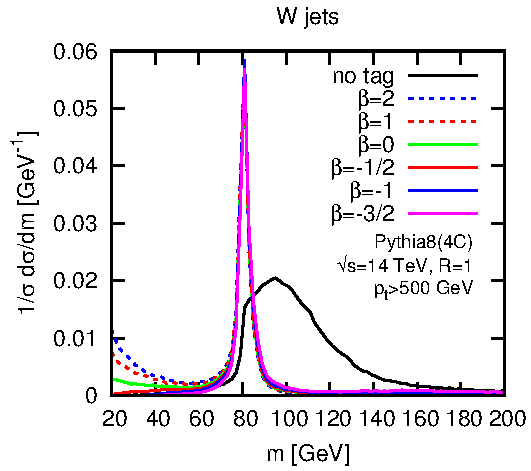
\includegraphics[width=.495\textwidth]{figures/Wtagging_W_spectrum.pdf}
    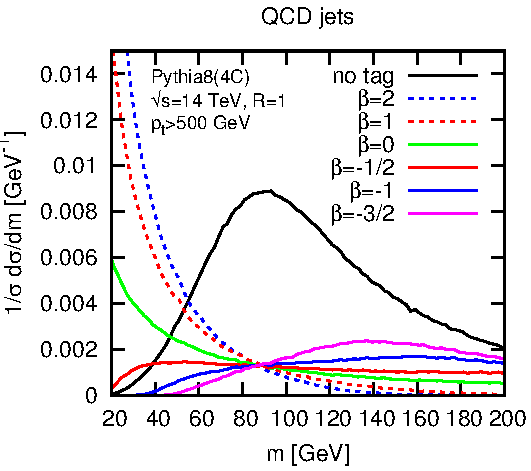
\includegraphics[width=.495\textwidth]{figures/Wtagging_j_spectrum.pdf}
  \end{center}
  \caption{Distributions of the jet mass in \W + jeta signal simulations (left) and multi-jet QCD background (right), before (in black) and after applying soft drop algorithm. Each curve corresponds to a different value of the parameter $\beta$.~\cite{Larkoski:2014wba}}
  \label{fig:softdrop_original}
\end{figure}

\noindent The net effect of the soft drop algorithm is studied in Monte Carlo simulations of a \W hadronic decay process (signal), in association with jets, and of a multi-jet QCD process (background). Jets are clustered with the anti-\kt algorithm with a parameter $R_0 = 1$ and asked to have $\pt>500$ \GeV and $|\mathcal{Y}|<4$. The parameter $z_{\text{cut}}$ is chosen such in a way that the number of events falling in the \W mass window ($[70,90]$ \GeV) is the 35\% of the total number of events. The results before (black curve) and after the application of soft drop algorithm (coloured curves, depending on the value of $\beta$) are presented in fig.~\ref{fig:softdrop_original}~\cite{Larkoski:2014wba}. In particular, by comparing the ungroomed jet mass (in black) with the mass groomed with a parameter $\beta = 0$ (adopted in this analysis and displayed with a green curve), the soft drop mass of the leading jet is a very narrow distribution peaking around the nominal \W window in the signal sample, whilst it is pushed at lower values in the background sample.

\vspace*{1\baselineskip}

\noindent The soft drop algorithm is used in association with the Pile Up Per Particle Identification algorithm (PUPPI)~\cite{Bertolini2014}, designed to combine detector informations in order to compute a local metric $\alpha$, that describes with a weight how likely it is that one particle is coming from the primary vertex or from a pile-up event. A fundamental feature exploited by the algorithm is the \pt spectrum of the primary vertex particles, expected to be harder than that of the pile-up ones.

\noindent The local shape $\alpha$ is defined as:

\begin{equation}
\alpha_i = \log{ \sum_{j \in \text{event}} \frac{p_{T,j}}{\Delta R_{ij}} \Theta \left( R_{\text{min}} \leq \Delta R_{ij} \leq R_0 \right)},
\label{eq:puppi_shape_def}
\end{equation}

\noindent where $\Theta$ is the Heaviside step function, $\Delta R_{ij}$ is the angular distance between the considered $i$ particle and the neighbour $j$ particle, laying  in a cone $R_0 = 0.4$ centered around $i$ direction, within a minimum distance $R_{\text{min}} = 0.0001$. Given the softer \pt spectra of pile-up particles, $\alpha_i$ is smaller when $i$ particle does not originate from the primary vertex.

\noindent The function
\begin{equation}
\chi_i^2 = \Theta (\alpha_i - \bar{\alpha}_{PU}) \frac{\left(  \alpha_i -  \bar{\alpha}_{PU}  \right)^2}{\sigma^2_{PU}}
\label{eq:puppi_chi2}
\end{equation}
\noindent estimates how much $\alpha_i$ fluctuates from the median of the pile-up local shape $\bar{\alpha}_{PU}$ (that has a variance $\sigma^2_{PU}$), and it is distributed like a $\chi^2$ with 1 degree of freedom. The PUPPI weight is defined as the cumulative $\chi^2$ distribution $F_{\chi^2\text{, 1 d.o.f.}}$,

\begin{equation}
w_i = F_{\chi^2\text{, 1 d.o.f.}} (\chi_i^2).
\label{eq:puppi_weight}
\end{equation}

\noindent If the local metric of a particle is distributed closely to the expected distribution of the pile-up, its weight is $w=0$. Large fluctuations are more likely related to non pile-up particles, and they receive a weight close to 1.  All the particles whose weights are smaller than 0.01 are removed from the jet clustering procedure.

\vspace*{1\baselineskip}

\noindent The default soft drop PUPPI jet mass suffers from a systematic shift from the expected value of about $\sim 10\%$, and from some residual dependence on the jet \pt. Further corrections to the jet mass have been applied:

\begin{enumerate}
  \item a \pt-dependent correction to account for a small shift in the generated vector boson mass, applied only on simulated samples,
  \item a \pt-$\eta$-dependent correction to the reconstructed jet mass, applied separately for jets in the barrel and endcaps regions.
\end{enumerate}

\noindent Fig.~\ref{fig:fatjet_pre_softdroppuppimass_ZZ}-~\ref{fig:fatjet_pre_softdroppuppimass_WZ} show the jet mass for hadronically decaying \W or \Z bosons in bulk graviton and \W' signal samples, before and after the correction, without applying any selections. In fig.~\ref{fig:fatjet_softdroppuppimass}, the distribution of soft drop PUPPI jet mass is shown for the expected backgrounds of the analysis (coloured histograms) and data (black markers), before and after the corrections.

\begin{figure}[!htb]
  \begin{center}
    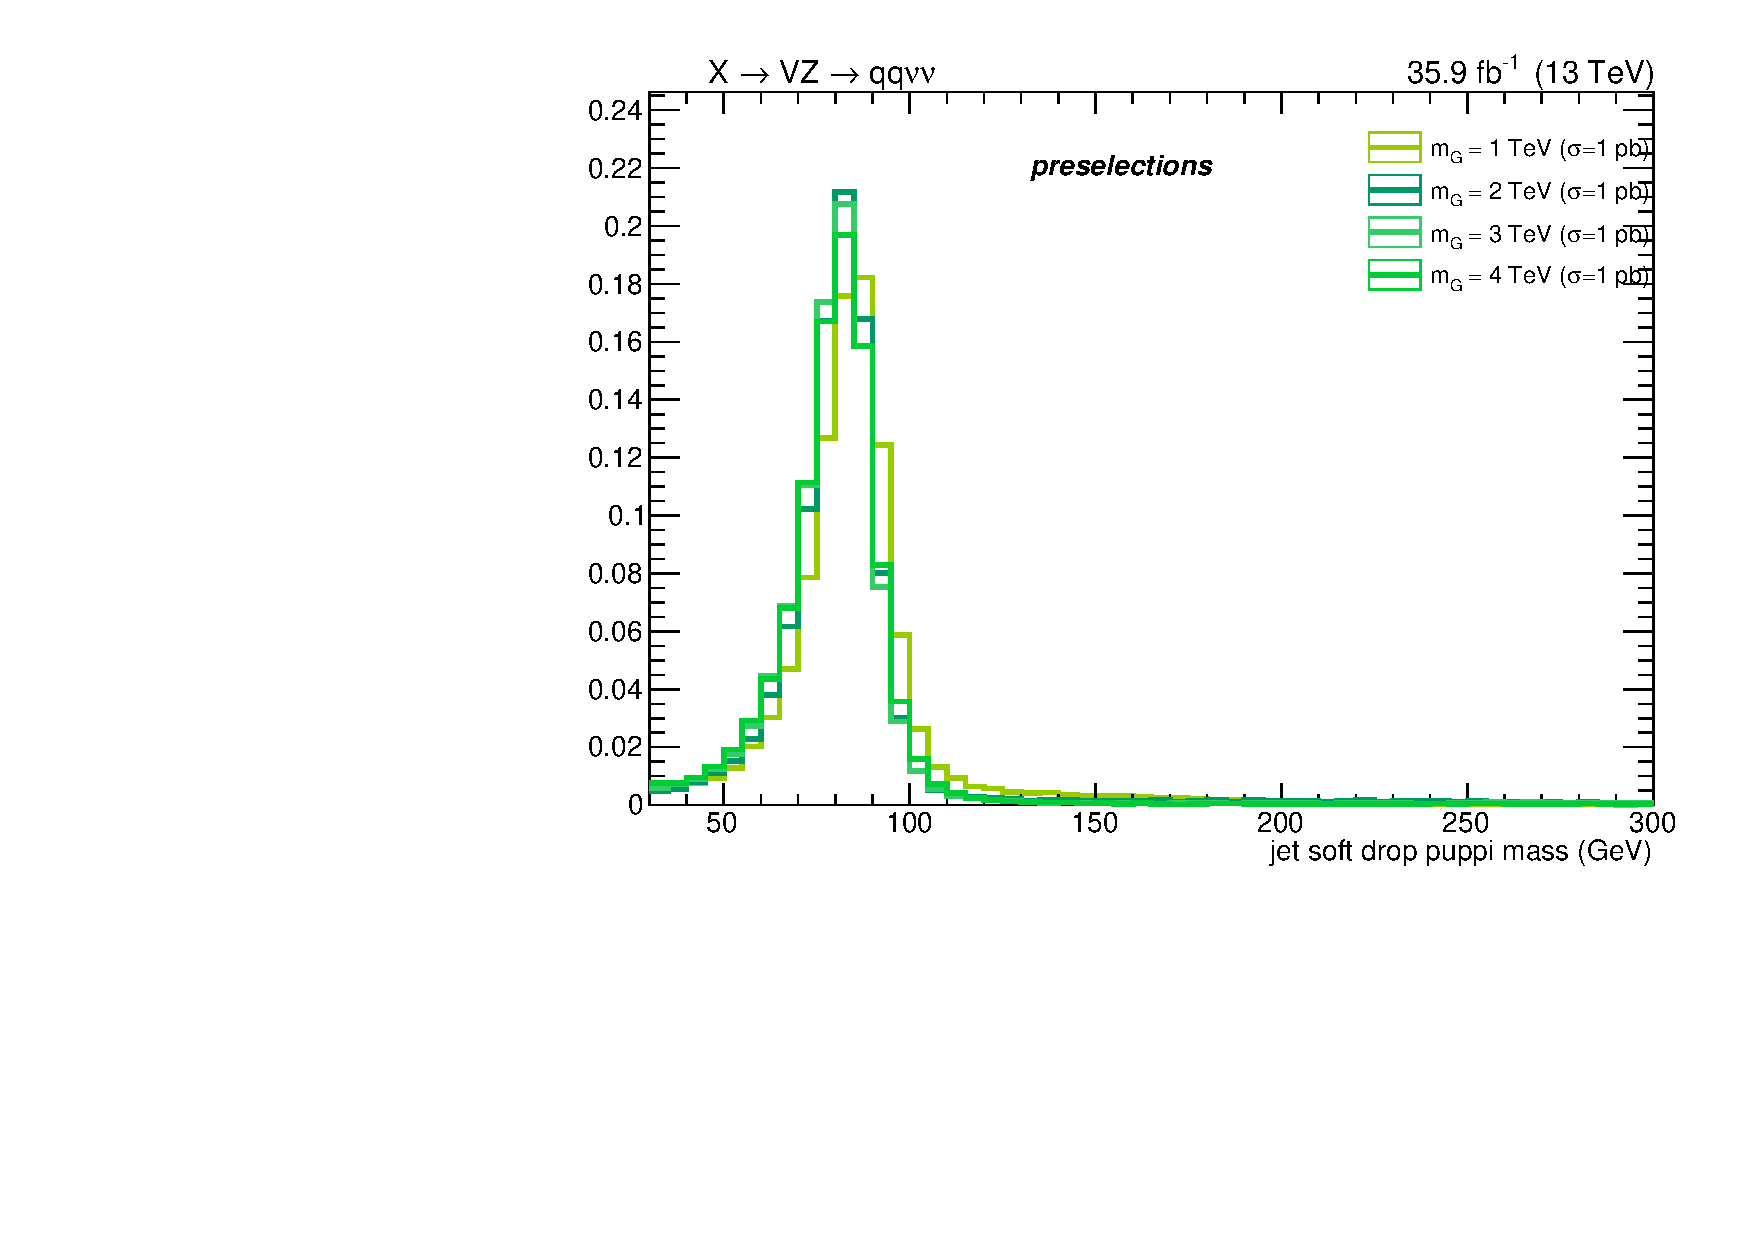
\includegraphics[width=.495\textwidth]{plots/v9_thesis/XVZnnPre/FatJet1_softdropPuppiMass_signalZZ.pdf}
    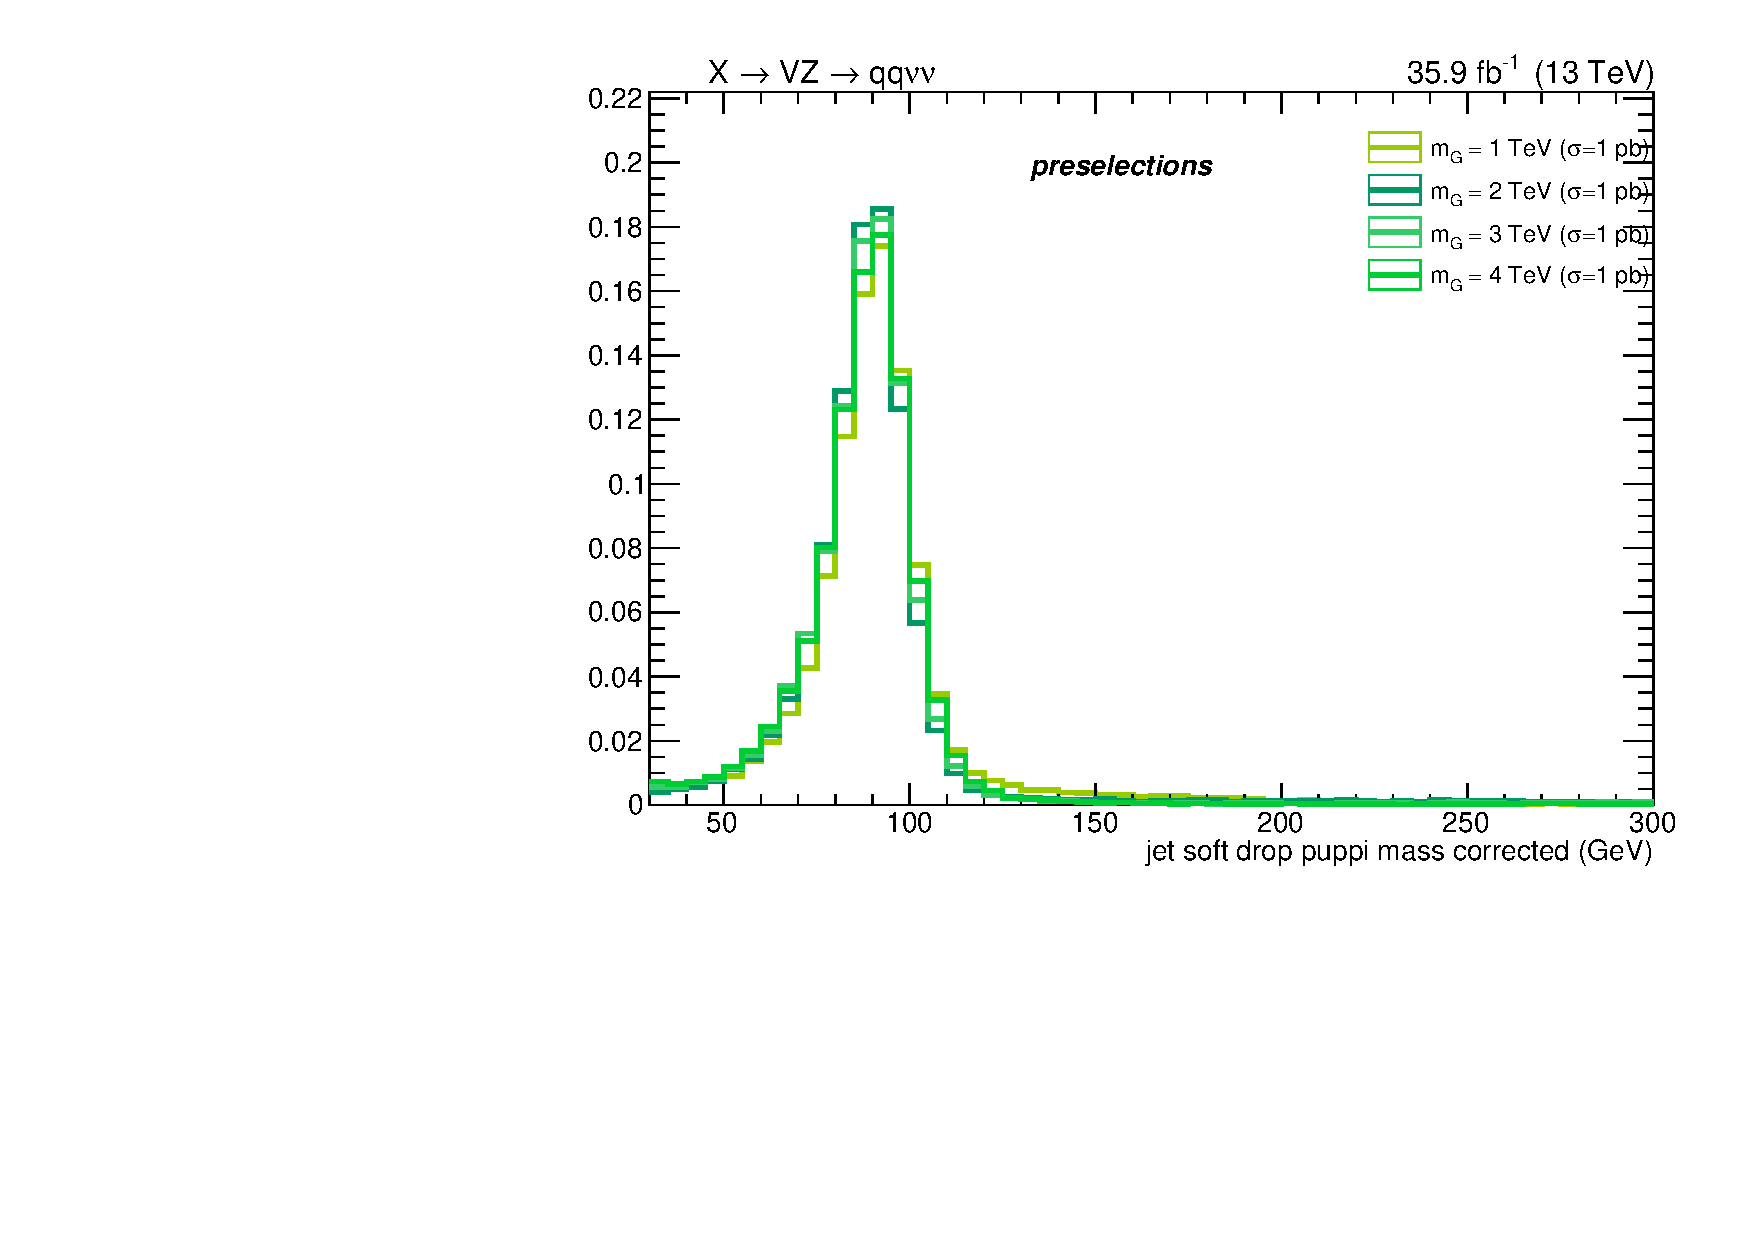
\includegraphics[width=.495\textwidth]{plots/v9_thesis/XVZnnPre/FatJet1_softdropPuppiMassCorr_signalZZ.pdf}
  \end{center}
  \caption{Soft drop PUPPI mass of AK8 jet reconstructed for different bulk graviton signal samples, before corrections (left) and after corrections (right).}
  \label{fig:fatjet_pre_softdroppuppimass_ZZ}
\end{figure}

\begin{figure}[!htb]
  \begin{center}
    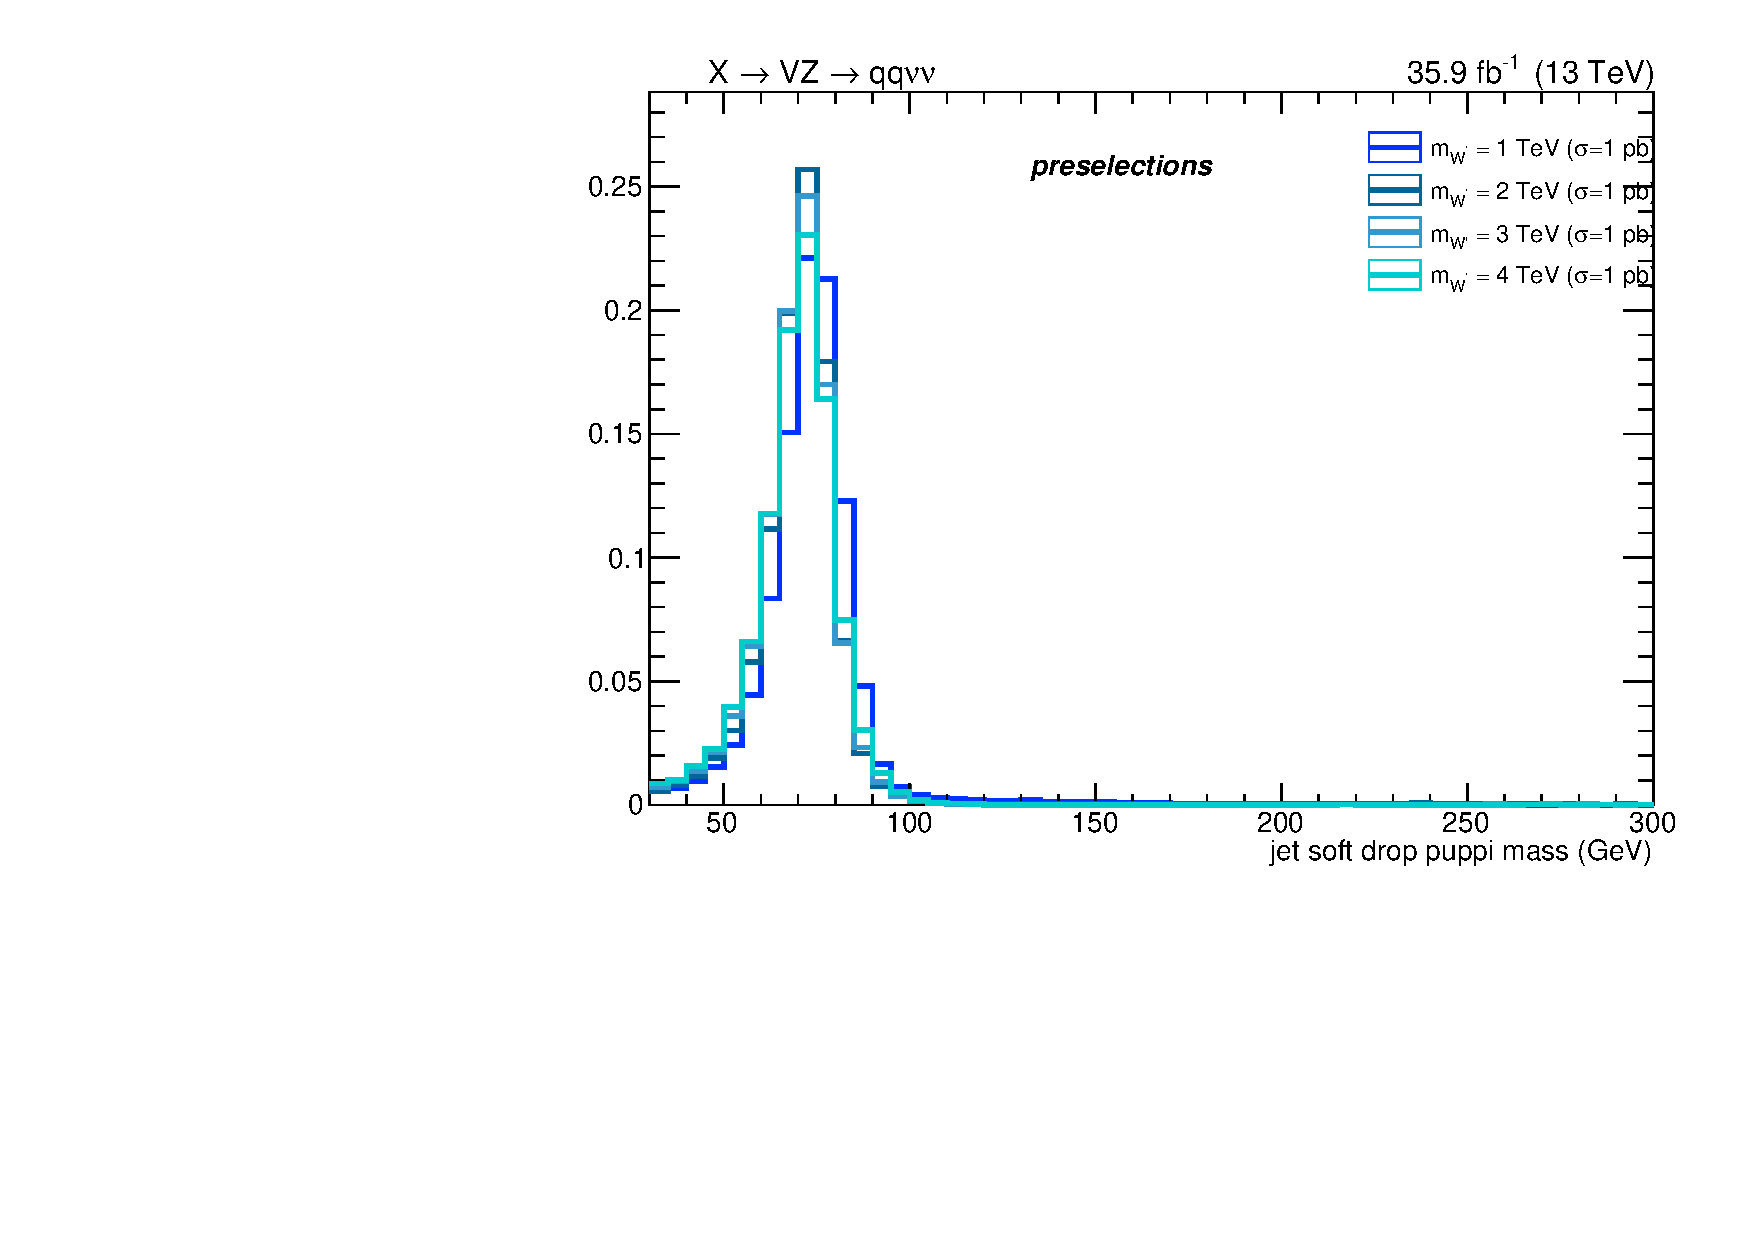
\includegraphics[width=.495\textwidth]{plots/v9_thesis/XVZnnPre/FatJet1_softdropPuppiMass_signalWZ.pdf}
    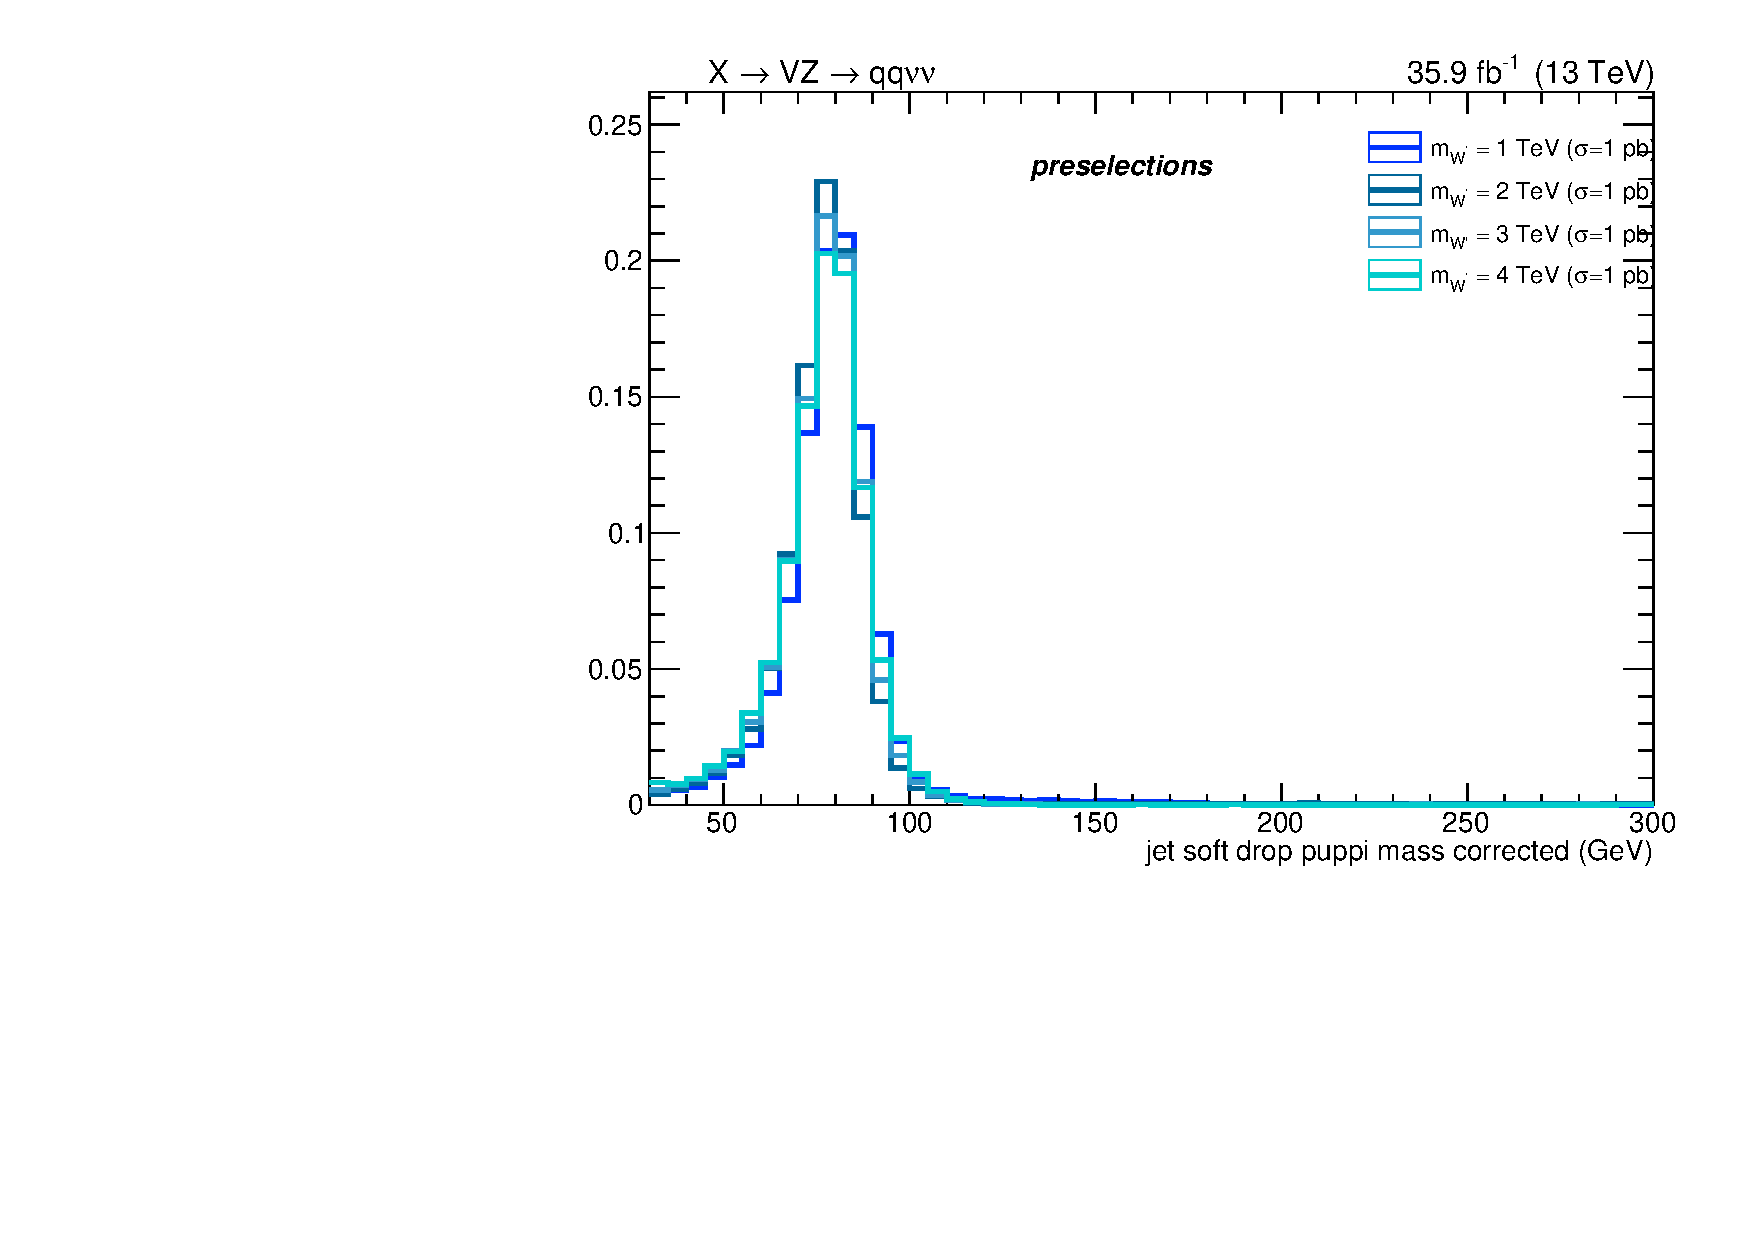
\includegraphics[width=.495\textwidth]{plots/v9_thesis/XVZnnPre/FatJet1_softdropPuppiMassCorr_signalWZ.pdf}
  \end{center}
  \caption{Soft drop PUPPI mass of AK8 jet reconstructed for different $W^{'}$ signal samples, before corrections (left) and after corrections (right).}
  \label{fig:fatjet_pre_softdroppuppimass_WZ}
\end{figure}

\begin{figure}[!htb]
  \begin{center}
    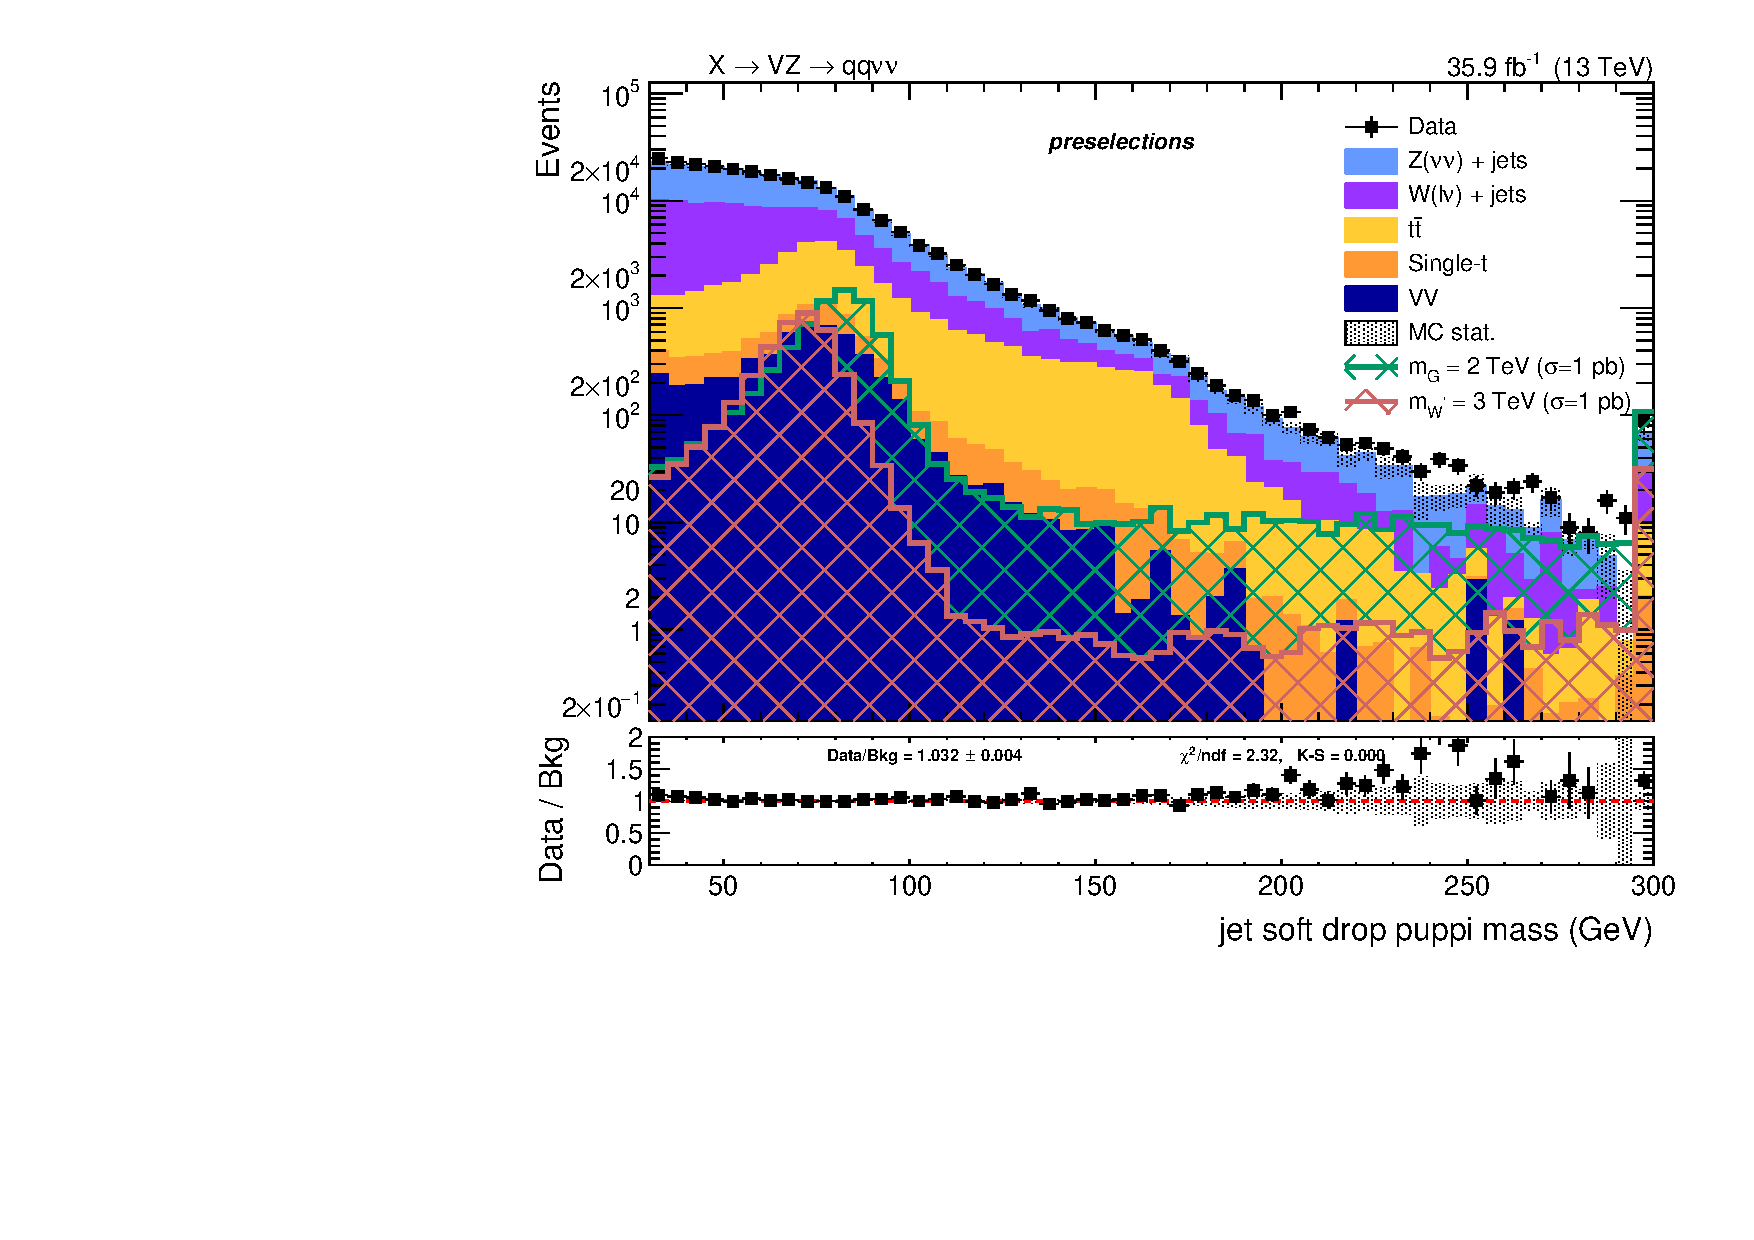
\includegraphics[width=.495\textwidth]{plots/v9_thesis/XVZnnPre/FatJet1_softdropPuppiMass.pdf}
    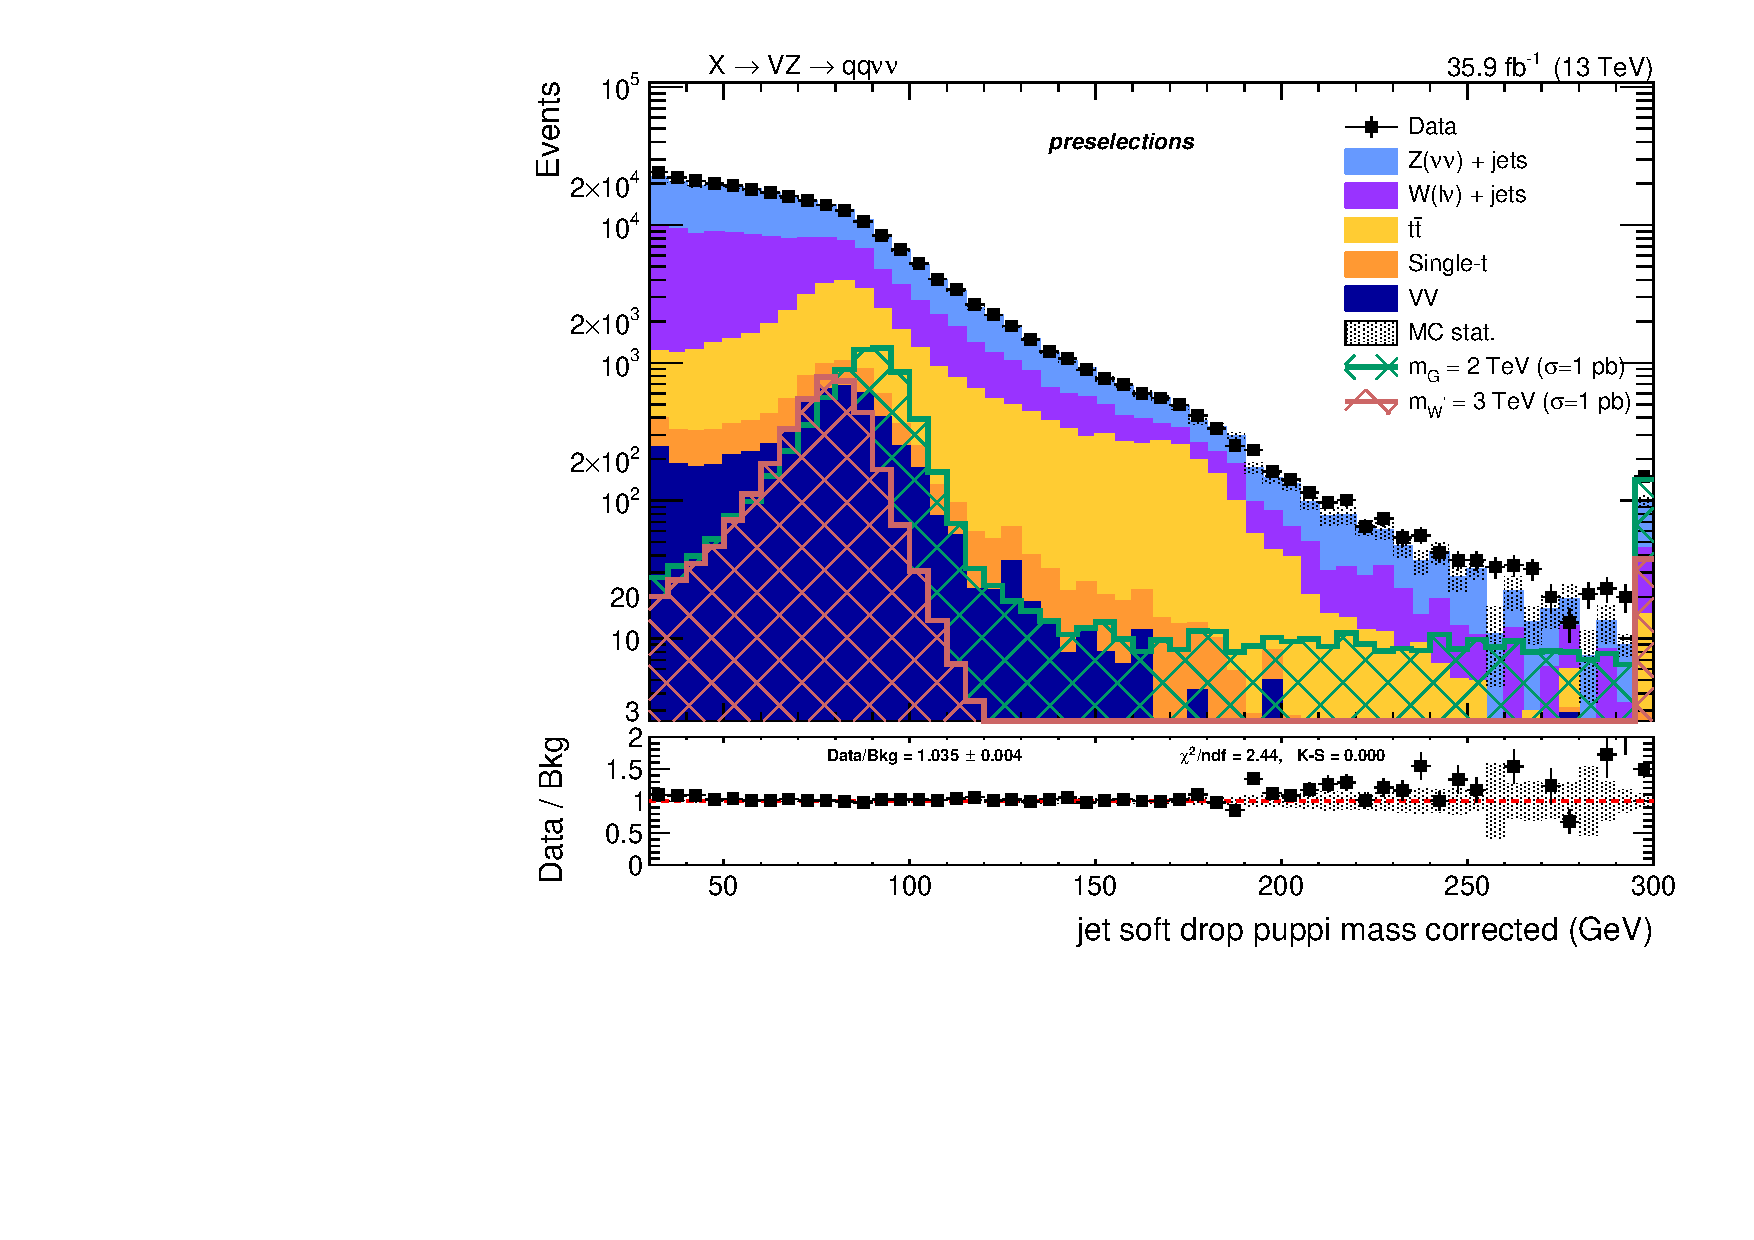
\includegraphics[width=.495\textwidth]{plots/v9_thesis/XVZnnPre/FatJet1_softdropPuppiMassCorr.pdf}
  \end{center}
  \caption{Soft drop PUPPI mass of AK8 jet; left: before corrections. right: after corrections.}
  \label{fig:fatjet_softdroppuppimass}
\end{figure}

\noindent In order to obtain a better data-Monte Carlo agreement, a smearing procedure has been applied to the soft drop PUPPI jet mass, by using the stochastic method, with a constant smearing coefficent ($1.00 \pm 0.20$), that does not depend on jet pseudorapidity, if it is restricted to $|\eta|<2.5$.

\vspace*{1\baselineskip}

\noindent The selection applied on the jet mass is a crucial step of the analysis, and it has to fulfill three purposes: it has to provide the maximum signal significance (best compromise between signal efficiency and background reduction), it has to avoid overlaps with the Higgs boson mass window, and it has to provide a sufficient data and simulation statistics for the control regions (the regions outside the mass cut). The soft drop PUPPI mass variable is used to define the following regions:

\begin{table}[!htb]
  \begin{center}
\caption{Mass regions defined for the analysis.\label{tab:massregions}}
  \begin{tabular}{l|cccc}
  & low-sideband & \V-region & $H$-region & high-sideband \\
 \hline
 \hline
 $M_{J}$ & 30-65 GeV & 65-105 GeV & 105-135 GeV & $> 135$ GeV\\ 
 \end{tabular}
 \end{center}
 \label{tab:SR-SB}
\end{table}

\noindent The "signal region" (SR) refers to the \V-region, where the largest signal yield is expected. The "sidebands" (SB) refer to the low-sideband and high-sideband, where a negligible amount of signal is expected. Events with a jet mass value lower than 30 \GeV are discarded, because of the high background contamination. The jet mass distribution of the \V candidate, in the sidebands and in the signal region, is shown in fig.~\ref{fig:mj_paper}. If the soft drop, PUPPI corrected mass of a large-con jet falls into the \V-region, the jet is defined as \V-tagged.

\begin{figure}[!htb]
  \begin{center}
    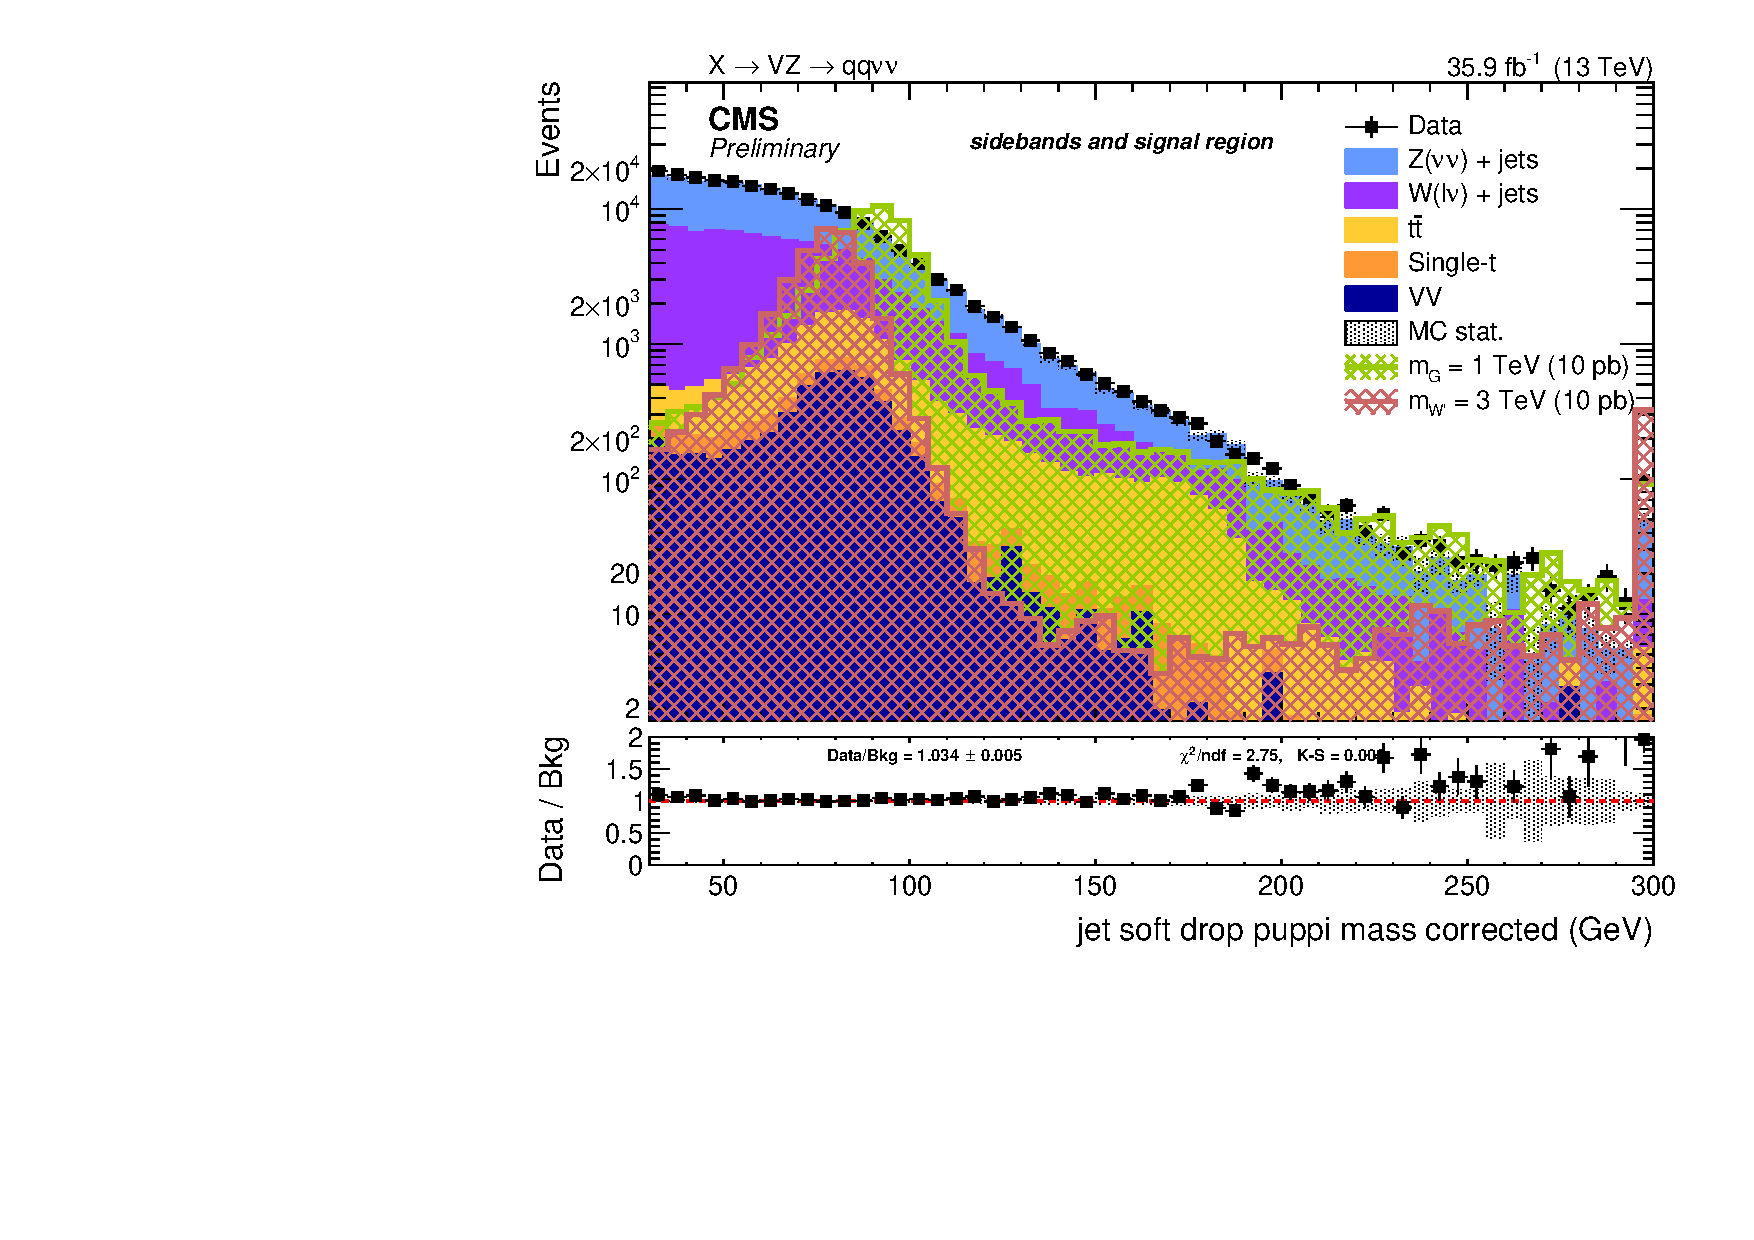
\includegraphics[width=.495\textwidth]{figures/FatJet1_softdropPuppiMassCorr.pdf}
  \end{center}
  \caption{Distribution of the soft drop PUPPI corrected mass of the leading AK8 jet, selected as the hadronically decaying \V candidate, in the sidebands and control region of the analysis, for expected SM background, bulk graviton signal, \Wp signal, and data.}
  \label{fig:mj_paper}
\end{figure}


\subsection{Jet substructure}\label{ssec:jetsub}

In order to further discriminate signal from background, the inner structure of the jet is investigated. Studying the distribution of the jet constituents with respect to the jet axis allows to test the hypothesis of the existence of multiple substructures, that could be an evidence of jets originated by more than one parton. The constituents of the considered jet are clustered again with the $k_T$ algorithm, and it is forced to return $n$ subjets. The $n$-subjettiness~\cite{Thaler2011}, $\tau_n$, is defined as

\begin{equation}
\tau_n = \frac{1}{d_0} \sum_k p_{T,k} \text{min} \left( \Delta R_{1,k}^\beta, \Delta R_{2,k}^\beta, \dots, \Delta R_{n,k}^\beta \right),
\label{eq:n_subjettiness_def}
\end{equation}

\noindent where $k$ labels the particles included in the jet, $p_{T,k}$ is the corrisponding transverse momentum of the $k$ constituent, and $\Delta R_{i,k}$ is the solid angle between the $k$ constituent and the $i$ subjet candidate. The parameter $d_0$ is a normalization factor:

\begin{equation}
d_0 = \sum_k p_{T,k} R_0,
\label{eq:n_subjettiness_d0}
\end{equation}

\noindent where $R_0$ is the clustering parameter of the considered jet. The $\tau_n$ variable describes to what degree a jet can be considered as composed by $n$ substructures; smaller values of $\tau_n$ correspond to higher compatibility to the $n$-prong hypotesis. A large-cone jet generated by the hadronic decay of an electroweak boson is expected to be a 2-prong object, whilst light flavour and gluon jets generated by colour interaction have a 1-prong monolithic structure. The $\tau_2$ or the $\tau_1$ alone, by the way, do not provide an optimal signal and background discrimination, as shown in fig.~\ref{fig:tau21_original_paper} (left and center); by looking at fig.~\ref{fig:tau21_original_paper} (right), it is clear that the most powerful discriminating variable is their ratio $\tau_{21} = \tau_2/\tau_1$:

\begin{equation}
\tau_{21} = \frac{ \frac{1}{d_0} \sum_k p_{T,k} \text{min}( \Delta R_{1,k}, \Delta R_{2,k} ) }{ \frac{1}{d_0} \sum_k p_{T,k} \Delta R_{1,k} }.
\label{eq:21_subjettiness_def}
\end{equation}

\begin{figure}[!htb]
  \begin{center}
    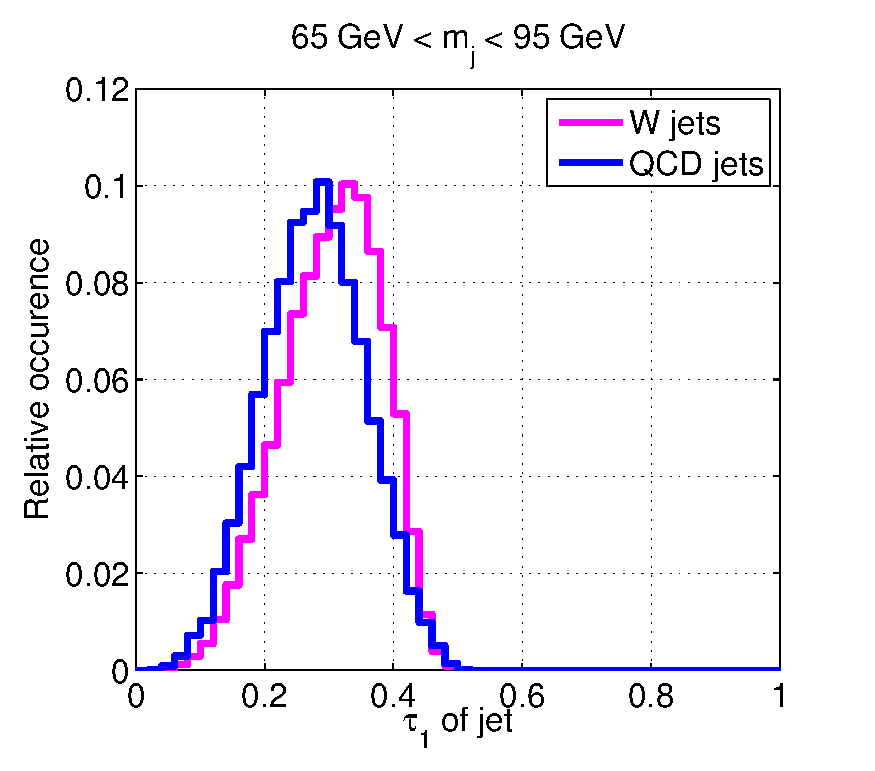
\includegraphics[width=.33\textwidth]{figures/tau1w.eps}
    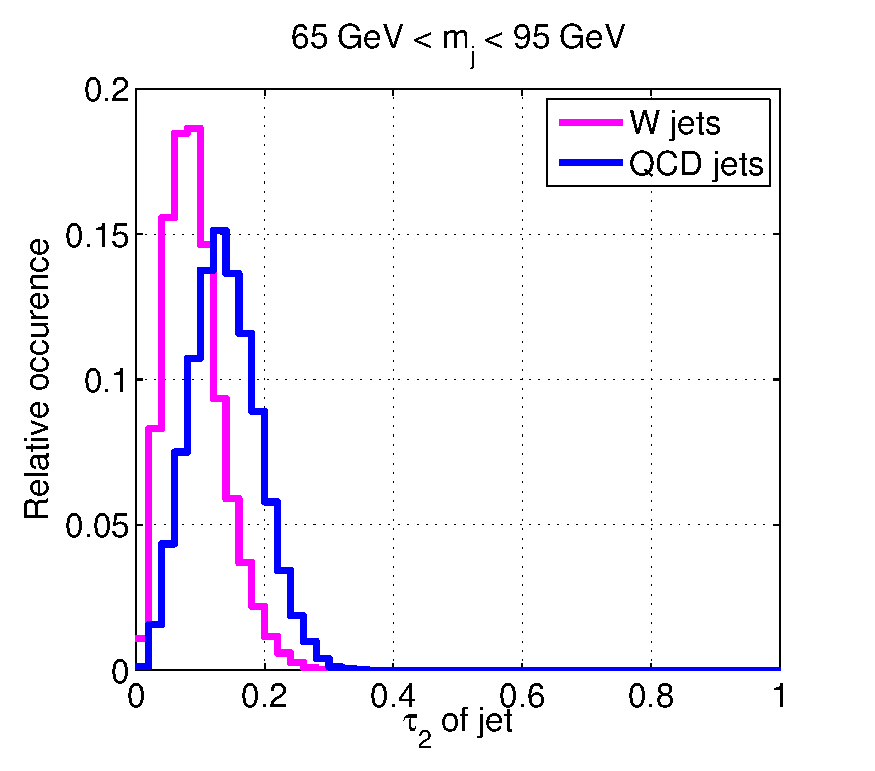
\includegraphics[width=.33\textwidth]{figures/tau2w.eps}
    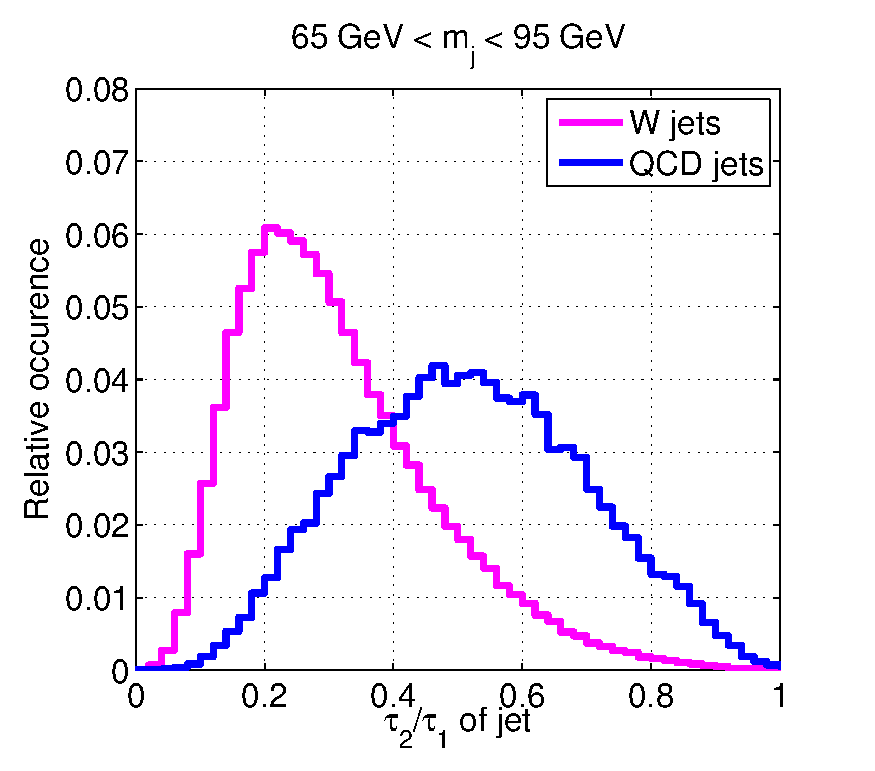
\includegraphics[width=.33\textwidth]{figures/tau2tau1w.eps}
  \end{center}
  \caption{Distribution of $\tau_1$ (left), $\tau_2$ (center), and $\tau_{21}$ (right) variables, in simulations of a \W plus jets process (in pink) and for a multi-jet QCD originated process (in blue). A selection on the leading jet mass is applied: $65 < m_j < 95$ \GeV; jets are clustered with a parameter $R_0 = 0.6$, $\pt > 300 \GeV$, $|\eta|<1.3$~\cite{Thaler2011}.}
  \label{fig:tau21_original_paper}
\end{figure} 

\noindent In fig.~\ref{fig:fatjet_pre_tau21}, the distributions of the $\tau_{21}$ variable are displayed for background and data, after applying the PUPPI algorithm (left), and for different bulk graviton mass hypoteses (right). The signal distribution is expected to peak at low values of the $\tau_{21}$ subjettiness variable.

\begin{figure}[!htb]
  \begin{center}
    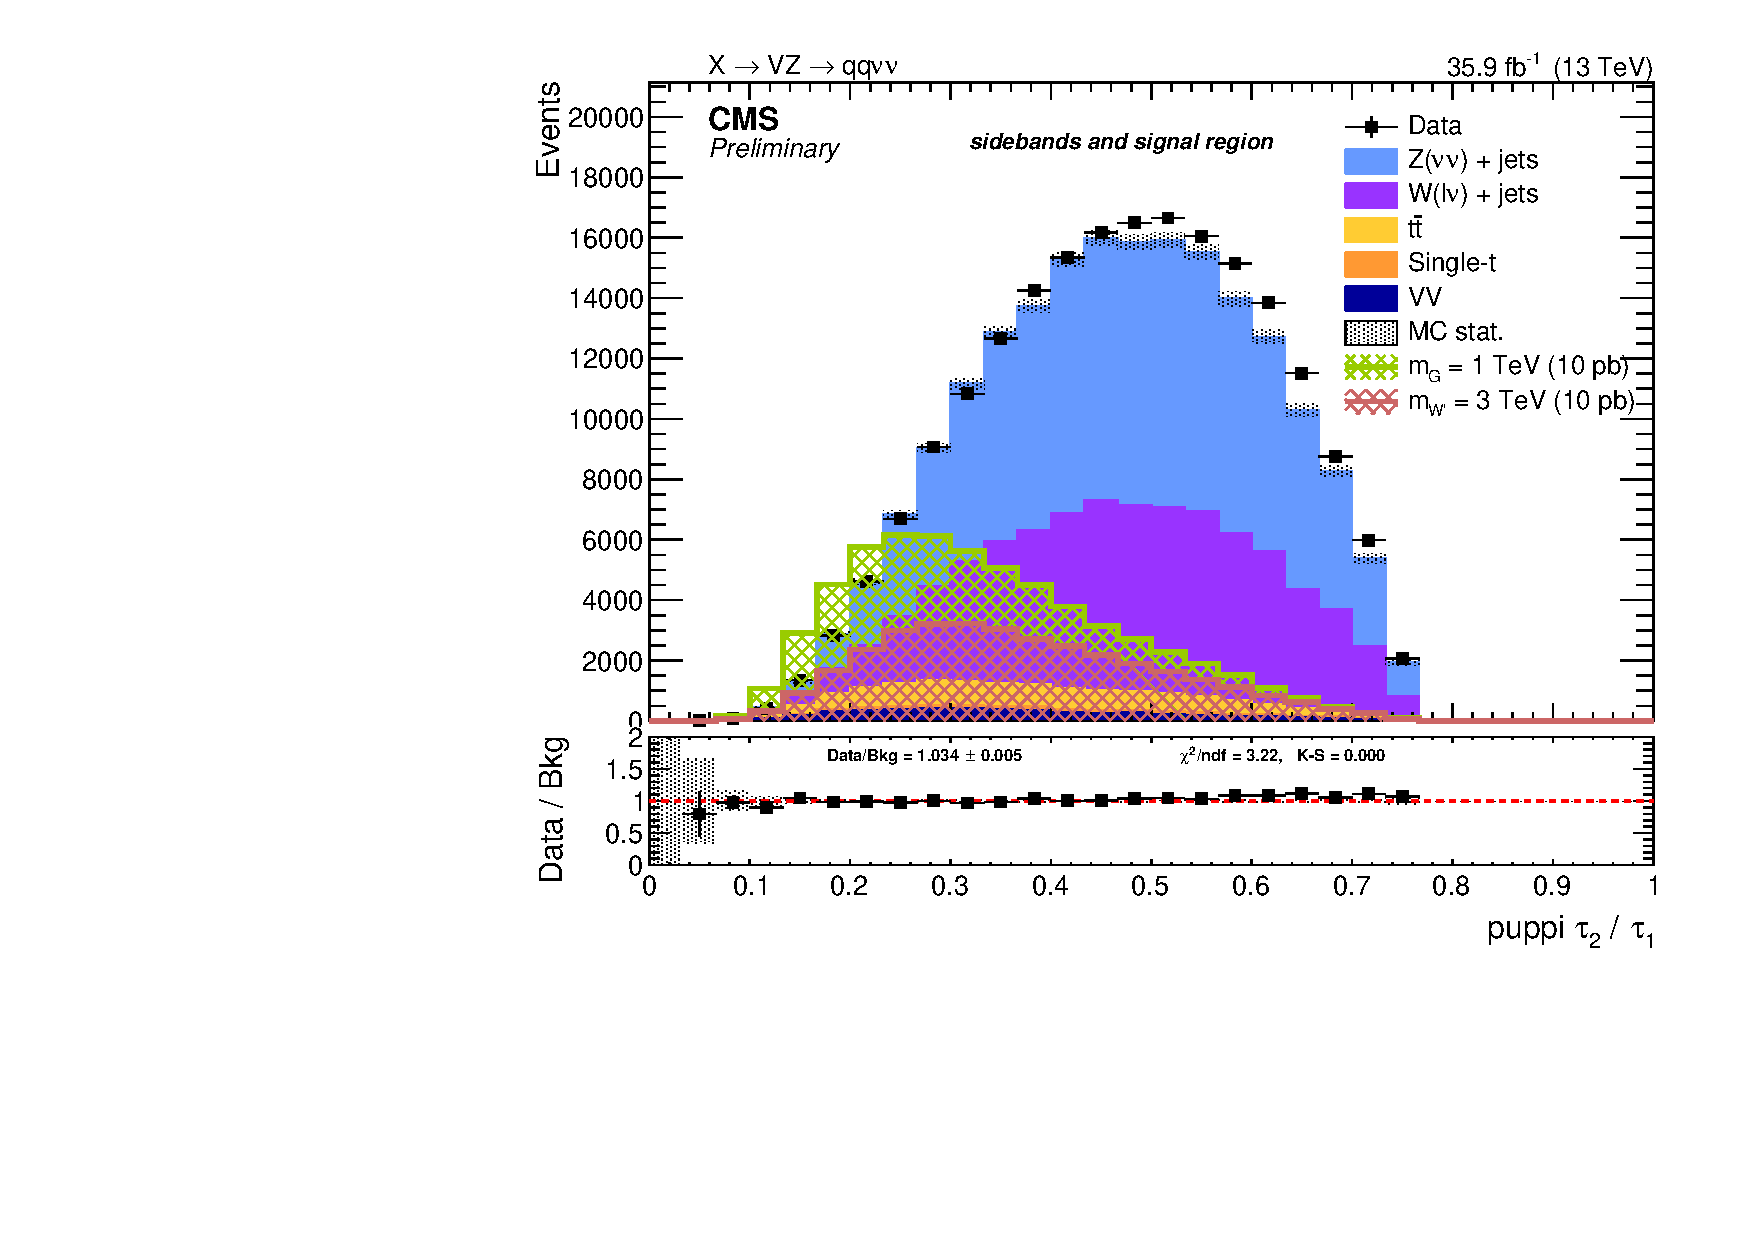
\includegraphics[width=.495\textwidth]{figures/FatJet1_puppiTau21.pdf}%
    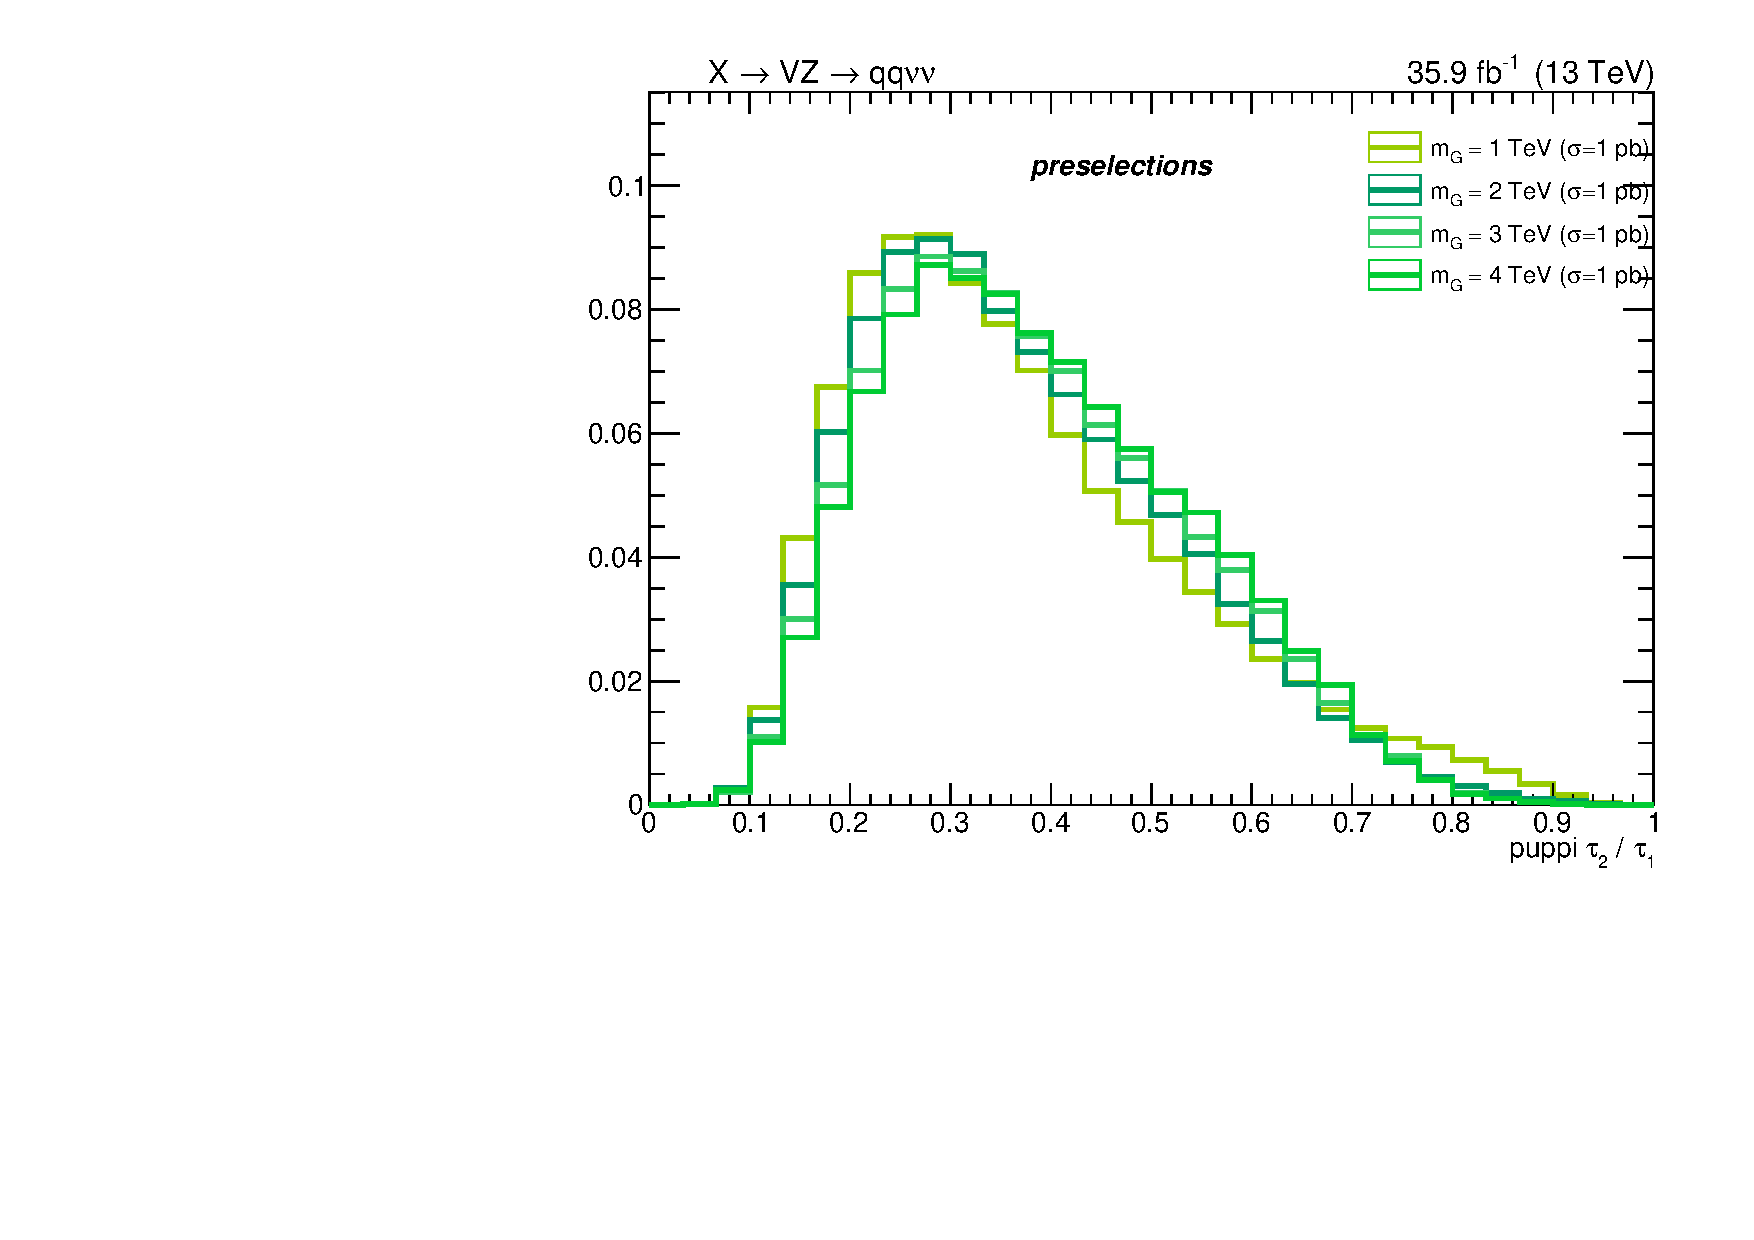
\includegraphics[width=.495\textwidth]{plots/v9_thesis/XVZnnPre/FatJet1_puppiTau21_signalZZ.pdf}
  \end{center}
  \caption{Distribution of the $\tau_{21}$ subjettiness of the leading AK8 jet, selected as the hadronically decaying \V candidate, for expected SM background and data (left), and for bulk graviton signal (right).}
  \label{fig:fatjet_pre_tau21}
\end{figure}

\vspace*{1\baselineskip}

\noindent The $\tau_{21}$ variable is used to classify the events into two exclusive categories, in order to improve the signal discovery reach. Events are included in either the high-purity ($\tau_{21} < 0.35$) or low-purity ($0.35 < \tau_{21} < 0.75$) category.


%[FIXME: SCALE FACTORS WILL BE UPDATED TO MORIOND17 ACCORDING TO THE 80X RECOMMENDATIONS FROM JMAR]
% The $\tau_{21}$ is a potentially discriminating variable (described in Section~\ref{ssec:jetsub}) between H-jets and QCD-jets, so a test to verify how much it can improve the signal significance is performed. The figure of merit is the same as the one described in Section~\ref{ssec:massopt}, and it is computed after applying pre-selection cuts, \V and \h \pt and mass cuts. A number of possible cuts are tested, ranging from $\tau_{21} < 0.3$ to $\tau_{21} < 0.7$, and compared between each other and the null cut option. Figure~\ref{fig:signal_tau21} shows the discriminating power of $\tau_{21}$ for all sources of SM background compared to the the signal, Higgs di-subjet decays. The significance for each selection is shown in Figure~\ref{fig:sign_tau21}, demonstrating that cutting on $\tau_{21}$ has no advantage  with the current luminosity. The $\tau_{21}$variable is therefore not used in the present analysis.

\noindent The choice of the $\tau_{21}$ categorization listed above is based on a study of the analysis sensitivity. Another $\tau_{21}$ categorization is probed, according to which events are grouped into different high-purity ($\tau_{21} < 0.40$) and low-purity ($0.40 < \tau_{21} < 0.75$) categories. This different set of $\tau_{21}$ cuts has been tested, along with that chosen for this analysis. Two figures of merit are considered: the discovery reach, namely the bulk graviton signal significance (displayed in fig.~\ref{fig:test_significance}), and the expected exclusion limit on cross-section times branching fraction at 95\% CL (displayed in fig.~\ref{fig:test_exclusion}), as a function of the reconstructed transverse mass of the resonance. To this purpose, the entire analysis workflow has been applied, performing an unbinned shape analysis with the analysis background estimation method, taking into account all the systematic uncertainties. In each figure, on the left, the figure of merit is plotted separately for each purity category, while in the right part of the figures the low and purity categories are combined together. Significance has been computed with a limited number of toys (100), hence the curves are non perfectly smooth, while the exclusion limit has been computed with the asymptotic formula. The procedures to extract signal significance and exclusion limits are described in sec.~\ref{sec:results}. Considering that the search region is 1-4 TeV, the choice of $0.35$-$0.75$ $\tau_{21}$ working points is legitimated.

 \begin{figure}[!htb]
   \begin{center}
     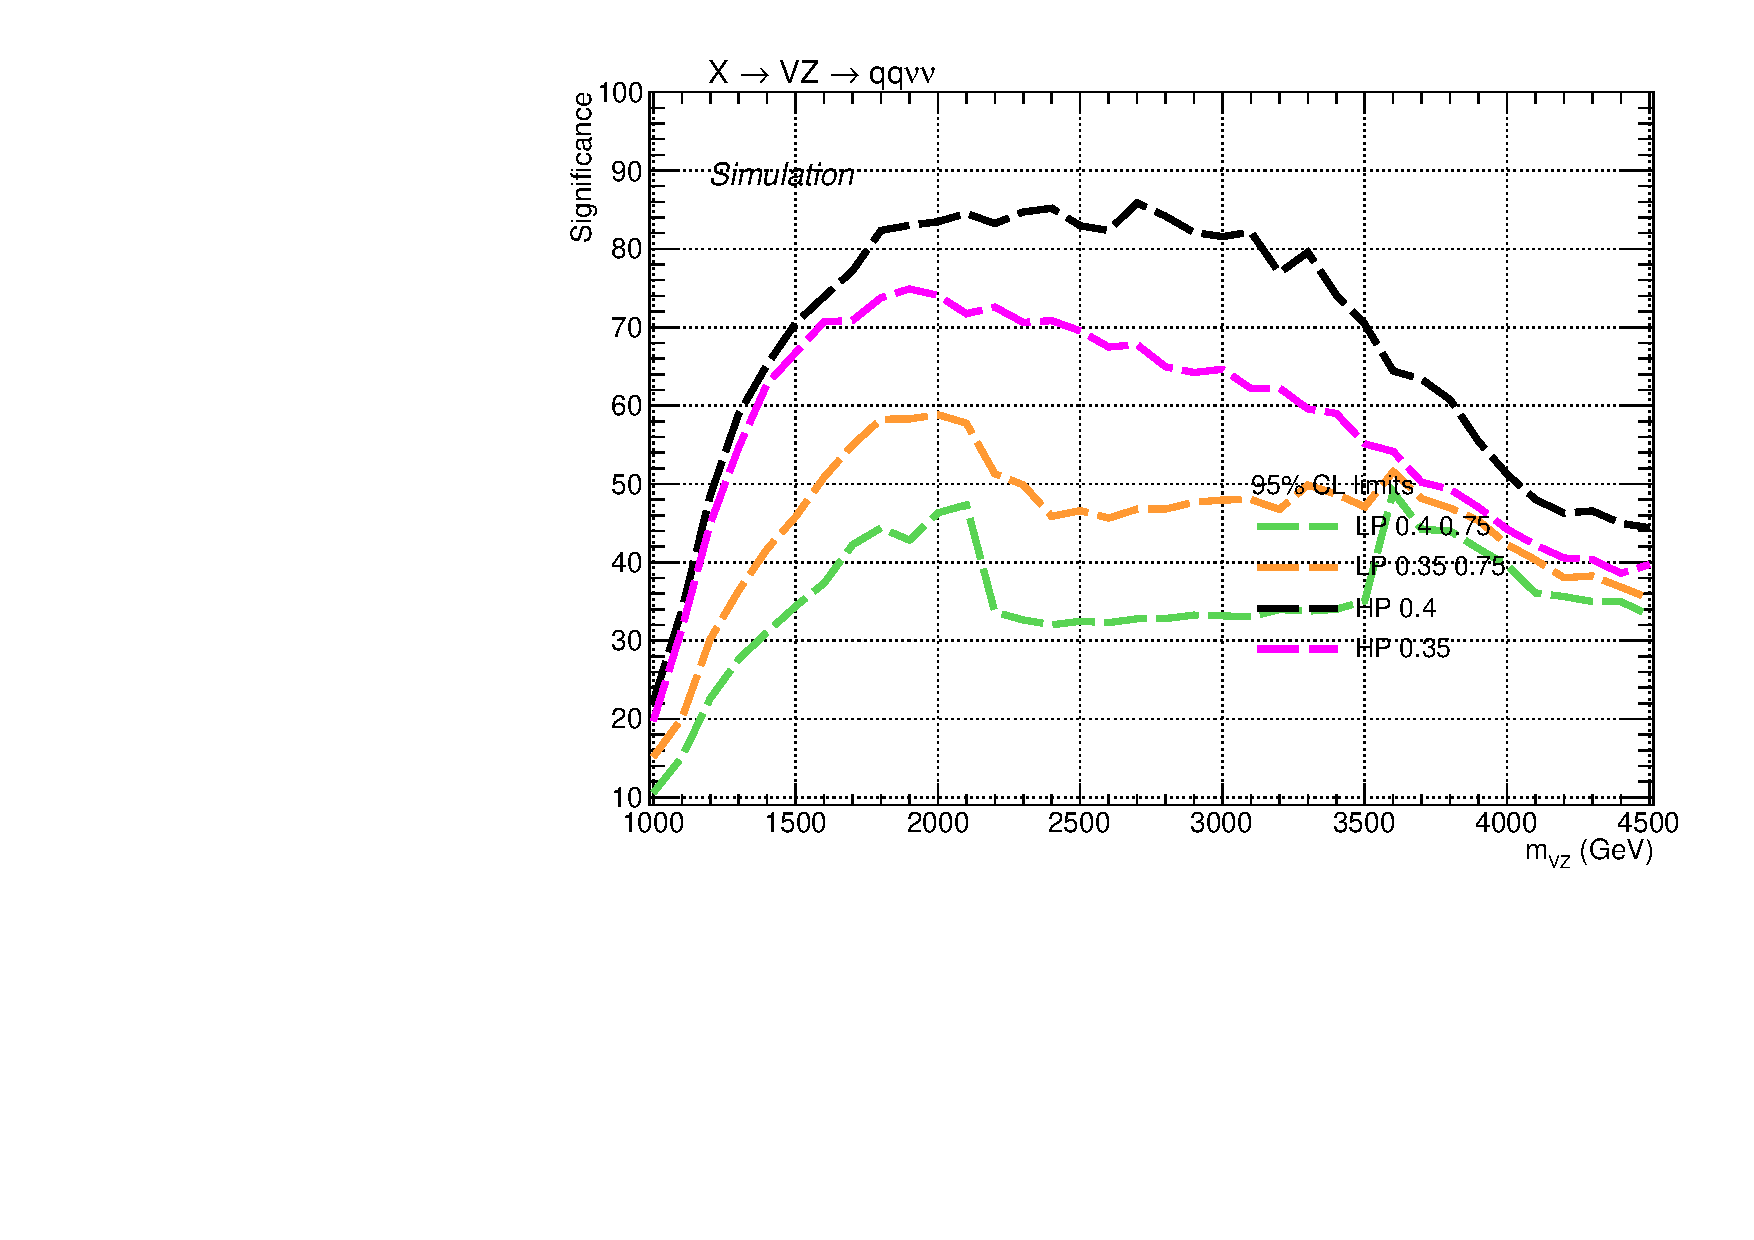
\includegraphics[width=.5\textwidth]{TestPurity/Significance_purityTest_LPHP_test_tesi.pdf}%
     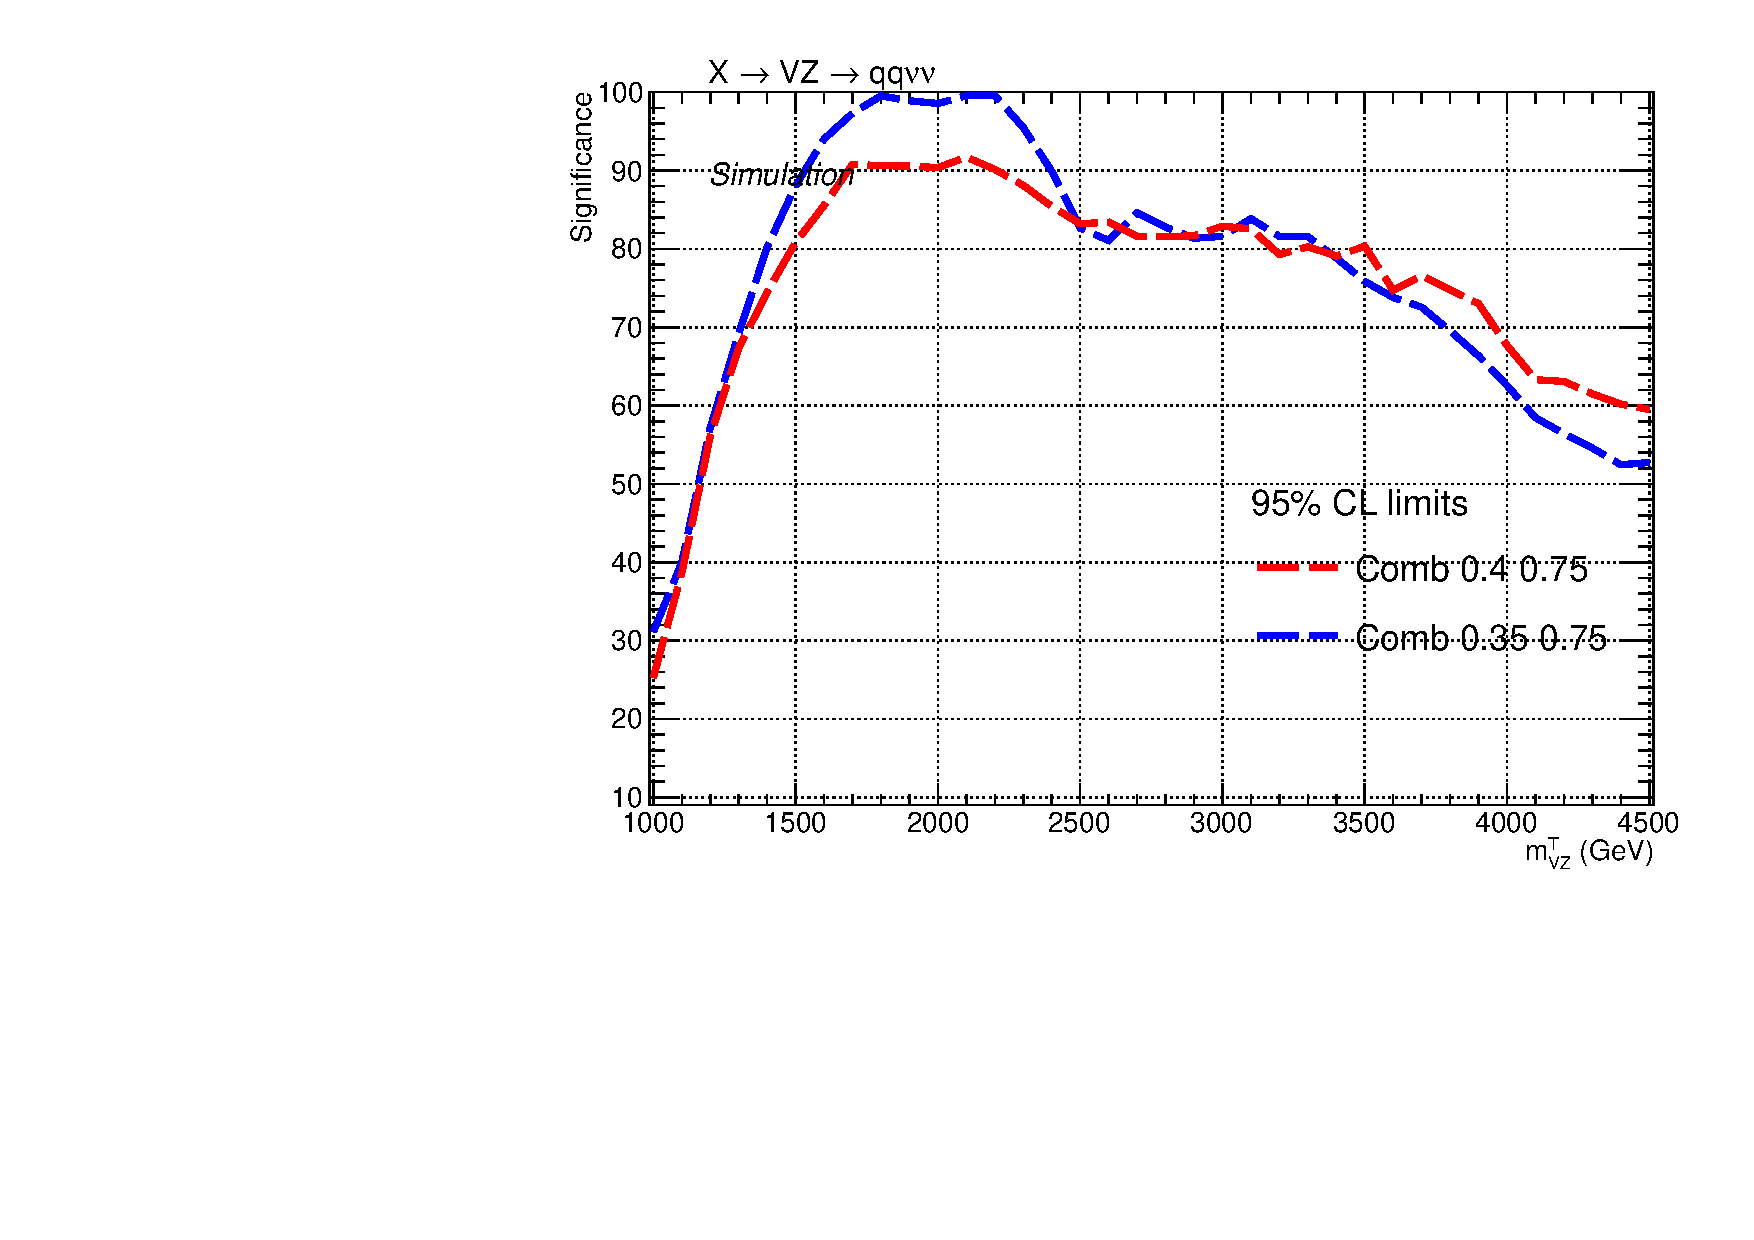
\includegraphics[width=.5\textwidth]{TestPurity/Significance_purityTest_comb_test_tesi.pdf}

   \end{center}
   \caption{Analysis sensitivity to bulk graviton signals, computed by applying different $\tau_{21}$ categorizations, considering the categories separately (left) and combining them together (right), as a function of the resonance mass.}
   \label{fig:test_significance}
 \end{figure}

 \begin{figure}[!htb]
   \begin{center}

     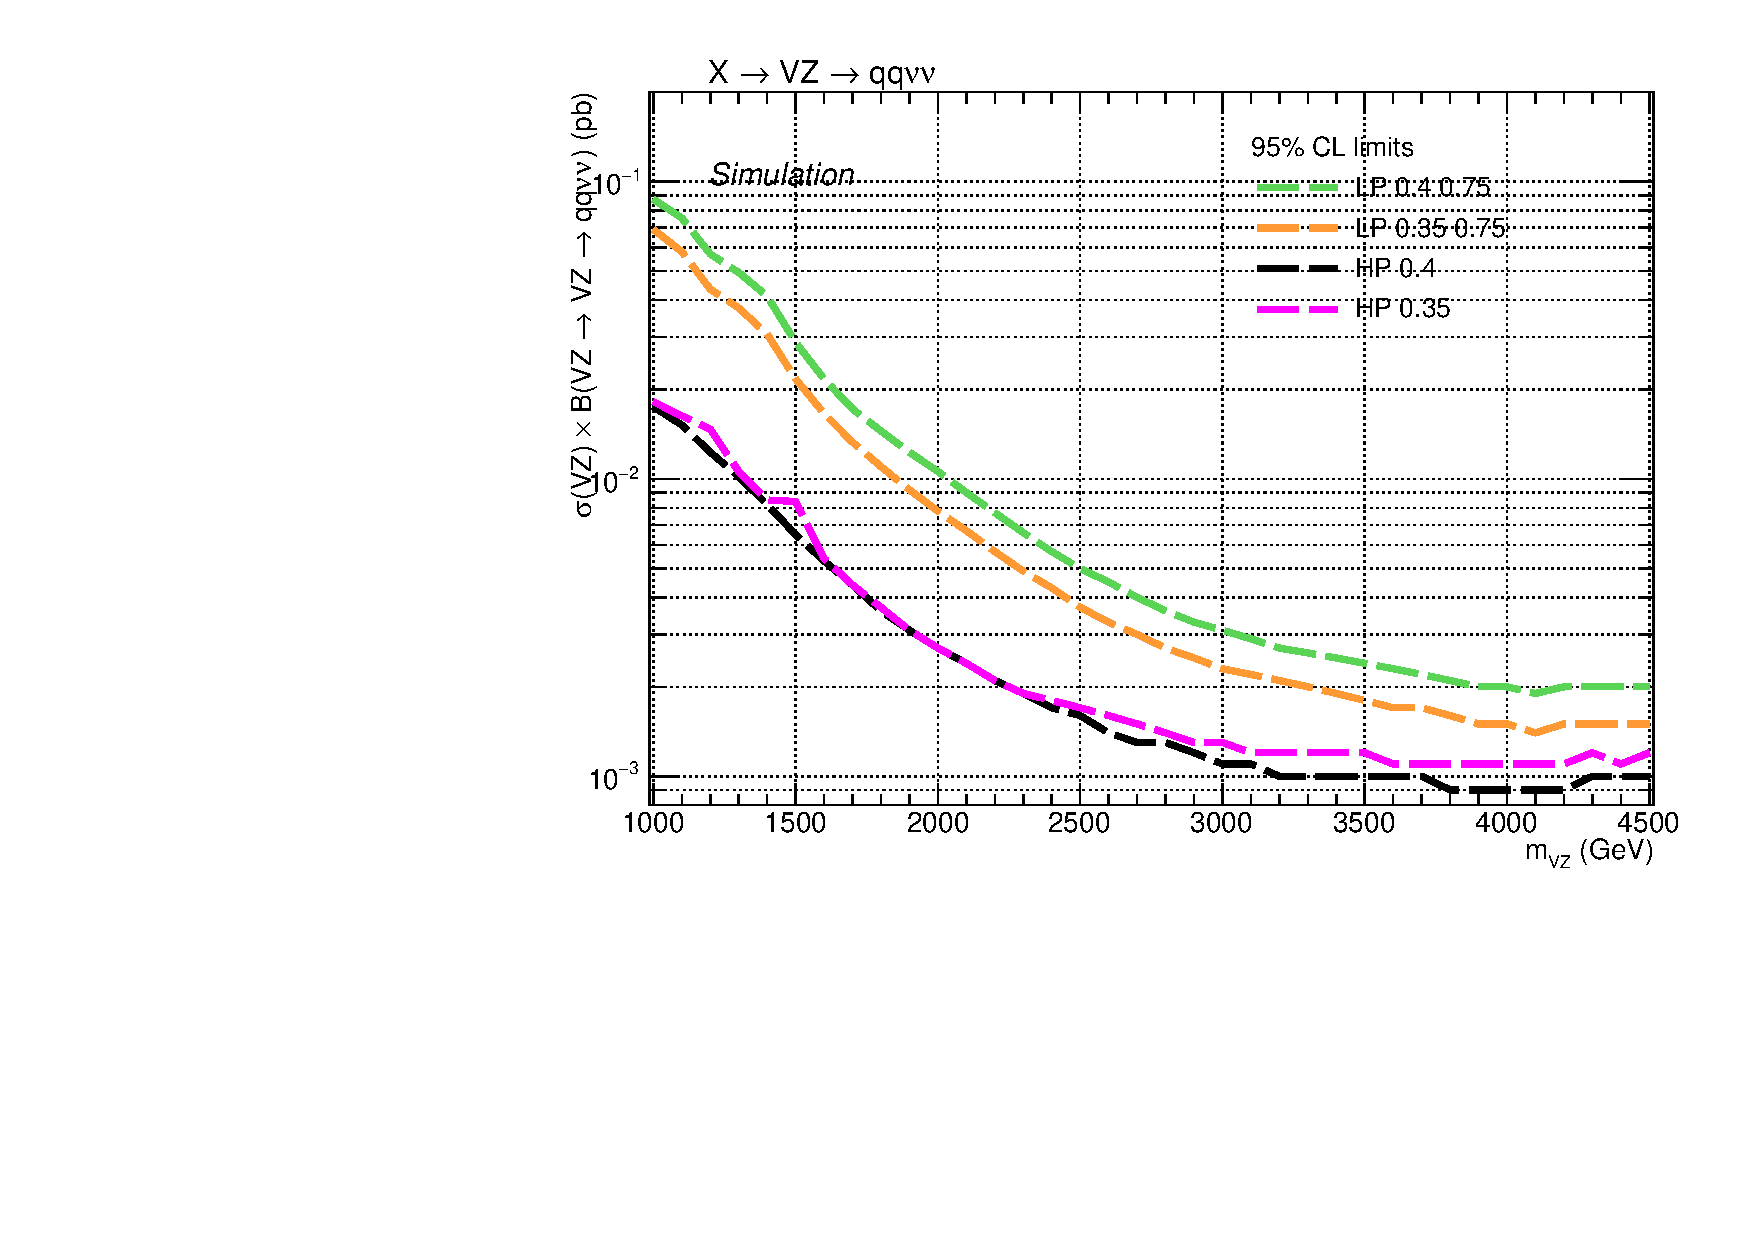
\includegraphics[width=.5\textwidth]{TestPurity/Exclusion_purityTest_LPHP_test.pdf}%
     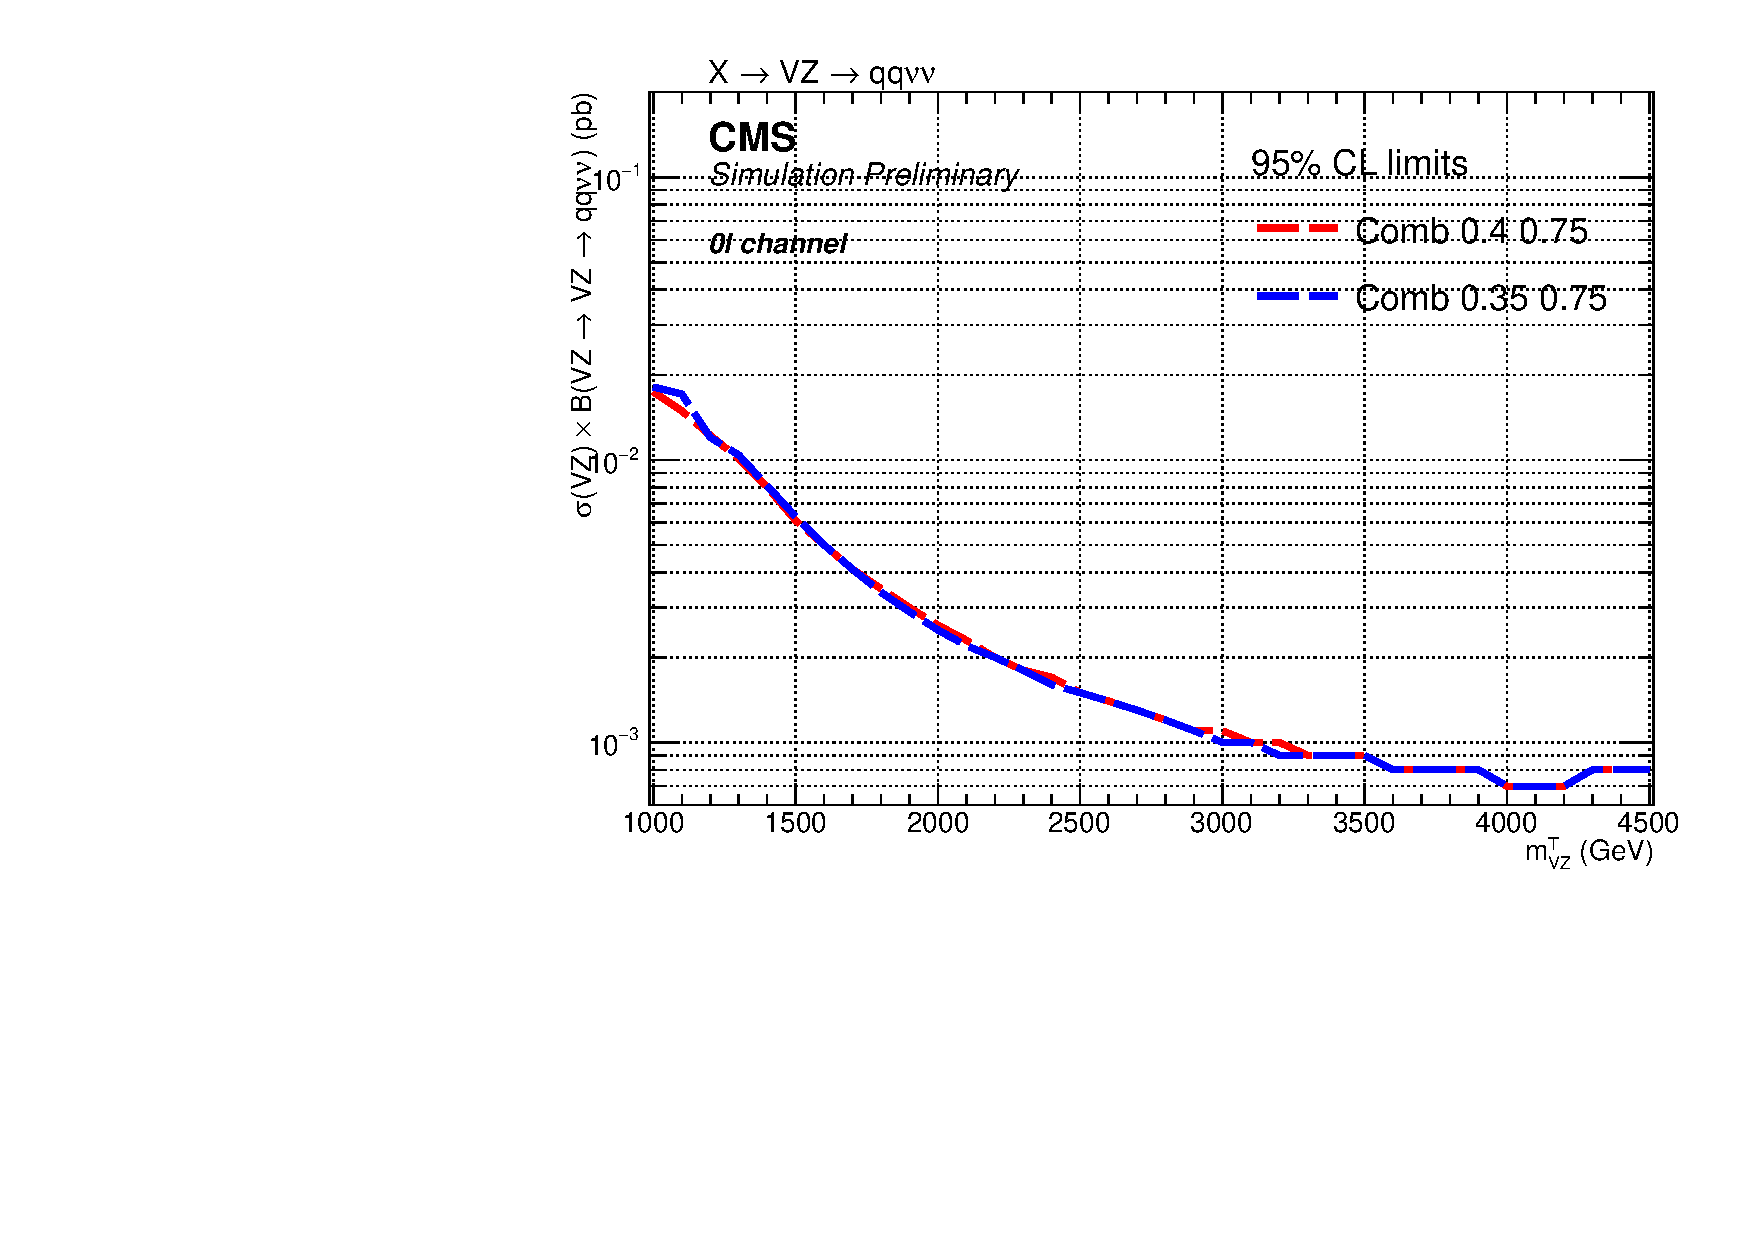
\includegraphics[width=.5\textwidth]{TestPurity/Exclusion_purityTest_comb_test.pdf}
   \end{center}
   \caption{Exclusion limit on cross-section time branching fraction at 95\% CL of bulk graviton signals, computed by applying different $\tau_{21}$ categorizations, considering the categories separately (left) and combining them together (right), as a function of the resonance mass.}
   \label{fig:test_exclusion}
 \end{figure}


\noindent When doing the $\tau_{21}$ categorization, \V-tagging scale factors have been taken into account to correct data and simulation discrepancies introduced by the $n$-subjettiness. They are described in sec.~\ref{ssec:jetsub_corr}.

\subsubsection{Corrections induced by jet substructure variables}
\label{ssec:jetsub_corr}
By applying a selection on the jet $\tau_{21}$, the jet mass spectrum is sculpted, hence the effects of the \V-tagging procedure shall take into account both the selections on mass and on substructure simultaneously. The distributions of the groomed jet mass and $\tau_{21}$ subjettiness have been compared in data and simulations, by selecting samples of di-jet, \ttbar and \W + jets events, and a significative discrepancy has been observed (10\%)~\cite{Khachatryan:2014vla}. Scale factors are extracted by selecting a \ttbar sample in data, because an high \pt \W boson is produced by the top quark decay. The hadronically decaying \W boson is tagged by choosing events where the soft drop mass of a large-cone jet lies in a window centered around the nominal \W mass. The jet mass distributions of events passing and failing the selection on the $\tau_{21}$ variable ($\tau_{21}<0.35$ and $0.35 < \tau_{21} < 0.75$, considered separately) are fitted simultaneously, both in data and in simulations. The \V-tagging scale factors are defined as the ratio of the $\tau_{21}$ categorization efficiencies in data and MC, and they are summarized in tab.~\ref{tab:tau21_sf}. The systematic uncertainties depend on the simulation of the \ttbar process, they cover the discrepancies observed while using different Monte Carlo simulations, and due to the choice of the fitting function.

\begin{table}[!htb]
  \centering
  \caption{Data-simulation scale factors, calculated on \ttbar samples, that correct the discrepancies related to the $\tau_{21}$ categorization.}
  \begin{tabular}{l|cc}
    $\tau_{21}$ selection & Purity category & Data-MC scale factor \\
    \hline
    \hline
    $\tau_{21}<0.35$ & high-purity & $0.99 \pm 0.11$ \\
    $0.35 < \tau_{21} < 0.75$ & low-purity & $1.03 \pm 0.23$ \\
  \end{tabular}

  \label{tab:tau21_sf}
\end{table}

\subsection{b-tagging}\label{ssec:btagging}
 
%The presence of a pair of b-quarks from the $\htobb$ decay is a very distinctive signature that permits a strong discrimination against all the backgrounds that involve jets with light flavors. The only  background which cannot be reduced with this technique is the $\Z$ production in association with one or two b-quarks, and the $\Z \to \bbbar$ decay which is also topologically similar to the signal. The latter can be only reduced by applying a jet mass cut, as described in Section~\ref{ssec:jetmass}.
% 

The presence of a b-tagged quark can be an hint to identify the top quark decays, representing a potential background to the search. The CSV b-tagging algorithm~\cite{Chatrchyan:2012jua} is applied to the AK4 jets. The jet is considered as tagged if the CSV discriminator value is above a threshold value; the b-tag efficiency is defined as the number of jets fulfilling this requirement, divided by the total number of jets. Since the purpose of the b-tagging is to reject the top quark events, the working point with the largest efficiency is chosen; the threshold of the CSV multivariate discriminant is listed in tab.~\ref{tab:btag}. 

%B-tagging algorithms are applied to both the fat-jet and the sub-jets, independently. For subjets, run-II taggers are by default applied on the same charged particle-flow candidate list that is used in the jet clustering (\emph{explicit jet-to-track association}). Thanks to the explicit jet-to-track association, the two sub-jets do not share any PF-constituent, avoiding unintended correlations.
% 
% 
%Several algorithms have been developed to tag jets from b-quarks. The recommended and best-performing algorithm is the {\tt pfCombinedInclusiveSecondaryVertexV2BJetTags}, often shortened to \emph{combined secondary vertex (CSV)}. This algorithm involves the use of secondary vertices, together with other lifetime information, like the IP significance or decay lengths. Secondary vertices are reconstructed with the inclusive vertex finder algorithm, that does not require jets (and thus is independent on the jet size) and uses all tracks to reconstruct secondary vertices~\cite{cms:JHEP032011136}. %In order to provide discrimination even when no secondary vertices are found, so the maximum possible b-tagging efficiency is not limited by the secondary vertex reconstruction efficiency ($50 \sim 60\%$). In many cases, tracks with an IP significance $> 2$ can be combined in a so-called pseudo vertex, allowing for the computation of a subset of secondary vertex based quantities even without an actual vertex fit. When even this is not possible, a no vertex category reverts simply to track based variables similarly to the jet probability algorithm. %The list of variables fed as input to an Artificial Neural Network is:
% \begin{itemize}
%   \item  the vertex category (real, pseudo, or no vertex)
%   \item  2D flight distance significance
%   \item  vertex mass
%   \item  number of tracks at the vertex
%   \item  ratio of the energy carried by tracks at the vertex with respect to all tracks in the jet
%   \item  the pseudo-rapidity of the tracks at the vertex with respect to the jet axis
%   \item  2D IP significance of the first track that raises the invariant mass above the charm threshold of 1.5 \GeV when subsequently summing up tracks ordered by decreasing IP significance
%   \item  3D signed IP significances for all tracks in the jet
%   \item  number of tracks in the jet
%   \item  $\Delta R$ between the secondary vertex flight direction and the jet axis
%   \item  number of secondary vertices associated to the jet or sub-jet
% \end{itemize}
 
% %In other words, the integral of the histogram from a certain discriminator cut up to infinity divided by the total number of jets.
%The typical b-tagging efficiency is between 40\% and 70\% while keeping the rate of mis-identified light-flavor jets between 0.1\% and 10\%. Three working points are usually defined for each algorithm, defining cuts in the discriminators based on the level of mis-tagging. The cut values and the corresponding mis-tagging for light-flavor jets relative to the CSV algorithm are reported in Table~\ref{tab:csvwp}.
% 
% \begin{table}[!htb]
%   \begin{center}
%   \begin{tabular}{lcc}
%   Working point & Cut & $\varepsilon_{light}$\\
%   \hline
%    Loose & 0.605  & $\sim 10\%$ \\
%    Medium & 0.890  & $\sim 1\%$ \\
%    Tight & 0.970  & $\sim 0.1\%$ \\
%   \end{tabular}
%   \end{center}
%   \caption{CSV official working points.}
%   \label{tab:csvwp}
% \end{table}

\begin{table}[!htb]
  \centering
  \label{tab:btag}
  \caption{Working point for CSV b-tagging algorithm.}
  \begin{tabular}{l|ccc}
     Working point & CSV discriminant threshold & tagging efficiency & mis-tag probability\\ 
    \hline
 \hline
     CSVL (Loose)  & $>0.5426$ & $\sim85\%$ & $\sim 10\%$  \\ 
     %CSVM (Medium) & $>0.8484$ & $\approx 1\%$   \\ 
     %CSVT (Tight)  & $>0.9535$ & $\approx 0.1\%$ \\ 
  \end{tabular}

  
\end{table}

\noindent Events where an AK4 jet, not laying in the AK8 jet cone, is b-tagged with the \emph{loose} working point threshold, are rejected. This veto allows to suppress the single-top events and \ttbar events by one half.

\noindent The b-tagging efficiency is not the same in data and MC. In order to take into account this difference, b-tagging scale factors for b-jets and mis-tagged light jets, measured for different physics processes, are calculated. A weight is extracted on a per-event basis, as a function of the b-tagging status of the jets and their kinematic variables~\cite{bib:btagsf}.

%With the b-tag veto, ST and TT bar are rejected....
%; this is a simple and effective method if there are a small number of possible combinations of jets and b-tagged jets.%Unfortunately, this is not the case of the present analysis. Other techniques allow to take into account the scale factors provided by BTV by \emph{reshaping} the discriminator output; this method has been already successfully applied in the SM VH analysis~\cite{bib:SMVH}, and is also described in detail in Ref.~\cite{bib:AZh,Khachatryan:2015lba}. The reshaping method does not sensibly increase the b-tagging scale factors uncertainty with respect to using single operating point SFs or other techniques used to apply the same scale factors.

\subsection{Missing Energy}
As pointed out in sec.~\ref{ssec:met_description}, Type-I corrected \MET is used in the analysis, along with dedicated filters to remove detector noise and events with bad reconstruction. In order to lie in the plateau of the trigger efficiency, $\MET > 200 \GeV$. Fig.~\ref{fig:type1_met} shows the \MET distribution for data and Monte Carlo after the corrections and filters.
 
 \begin{figure}[!htb]
   \centering
     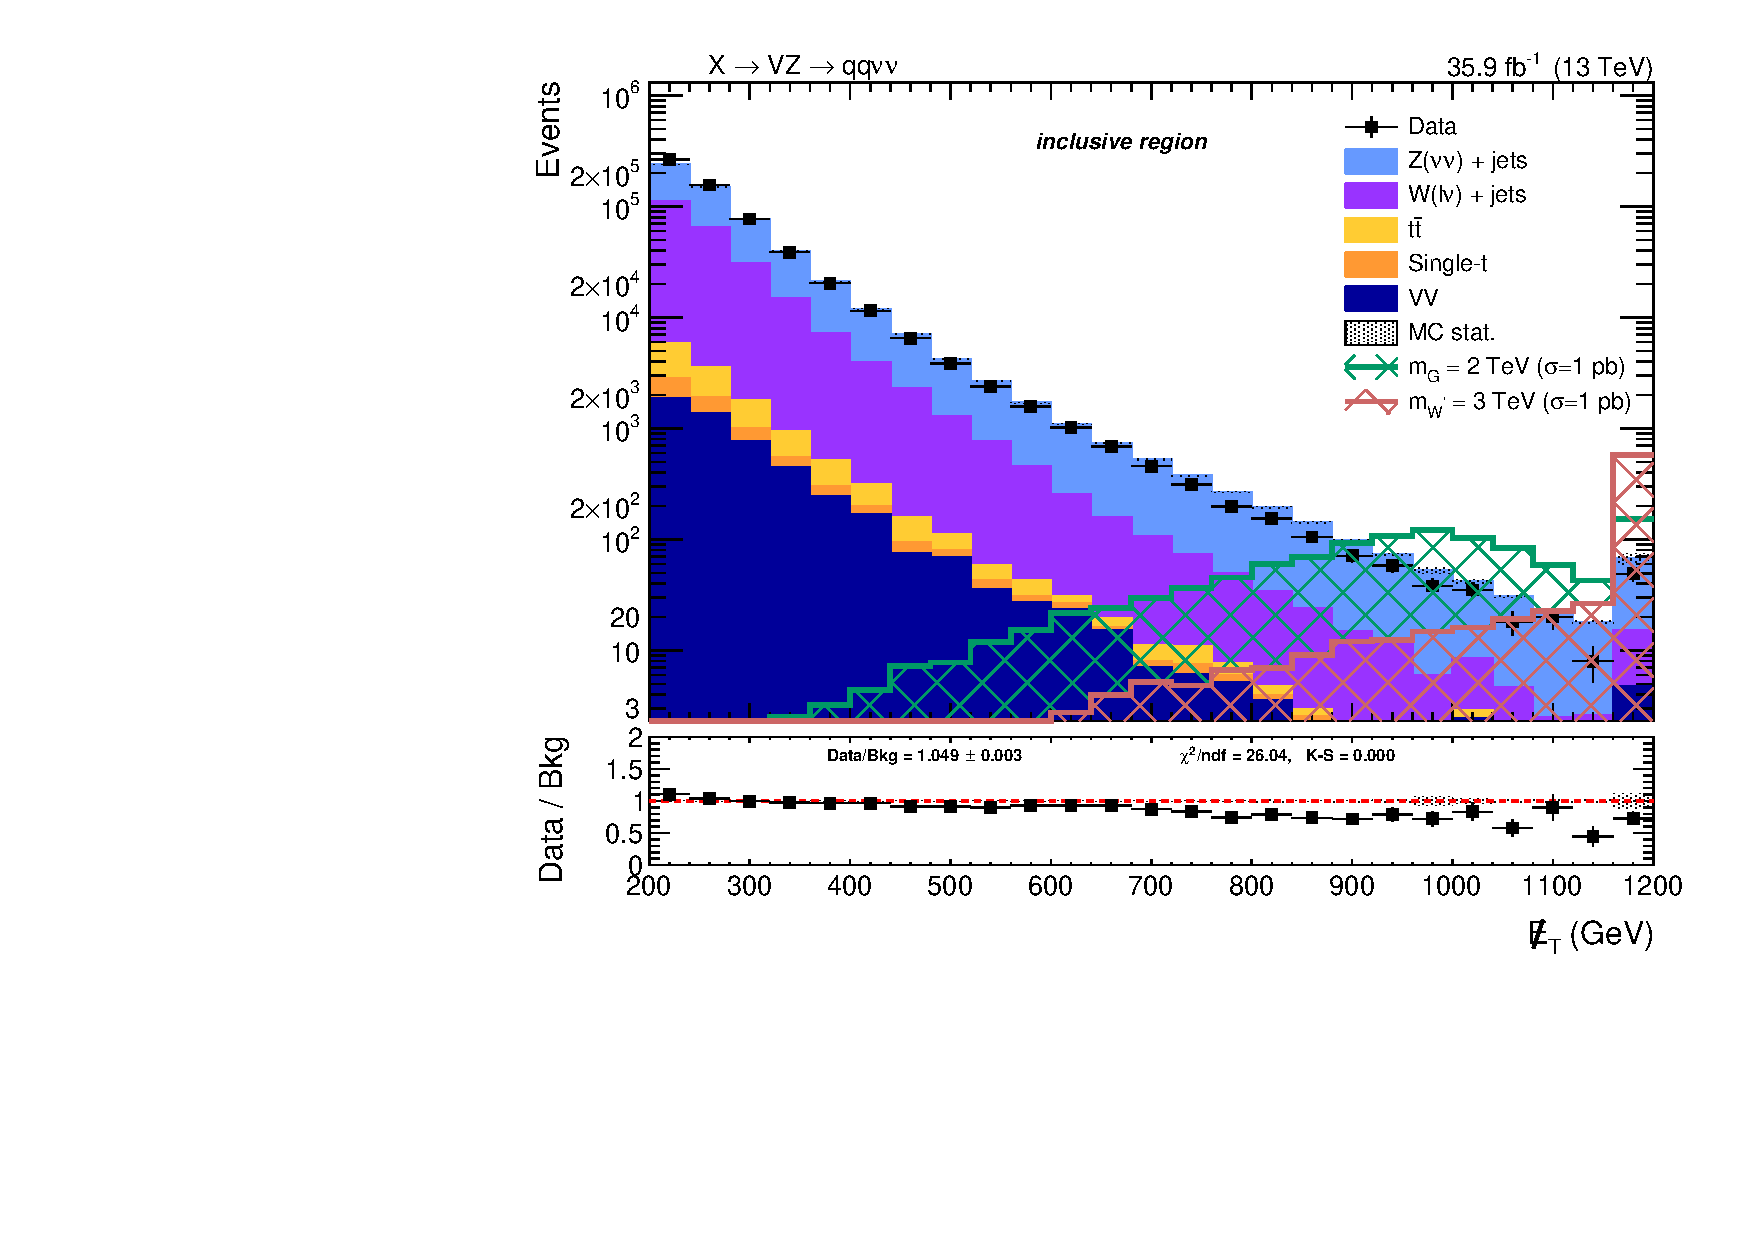
\includegraphics[width=.495\textwidth]{plots/v9_thesis/XVZnnInc/MEt_pt.pdf}
     %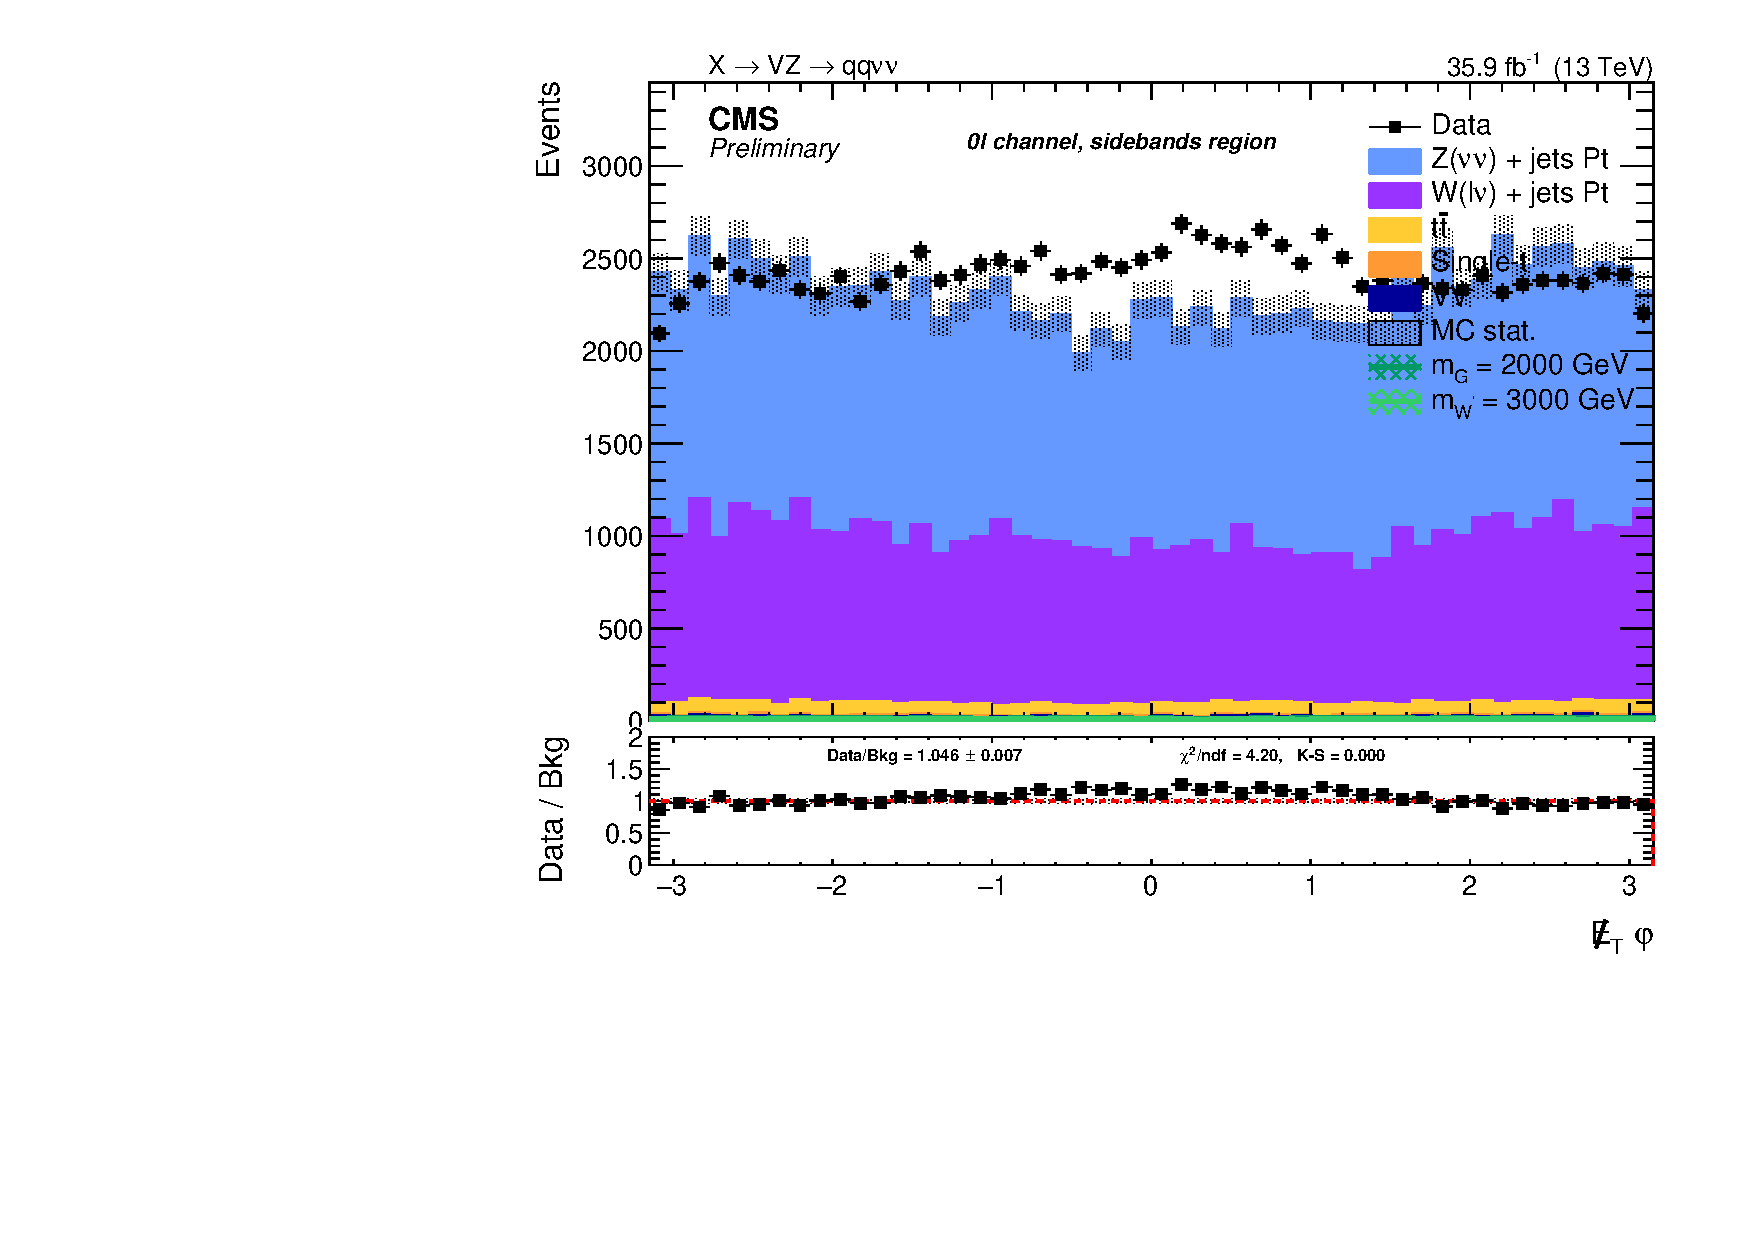
\includegraphics[width=.495\textwidth]{plots/v9_thesis/XVZnnInc/MEt_phi.pdf}
   
   \caption{Type-1 corrected \MET distribution after inclusive selections.}
   \label{fig:type1_met}
 \end{figure}


